\documentclass{tufte-book}

\hypersetup{colorlinks}% uncomment this line if you prefer colored hyperlinks (e.g., for onscreen viewing)

%%
% Book metadata
%\title{What's in the Bag for Latent Variable \\ \noindent Language Modelling?}
\title{To skip or not to skip: that's \{*\} question}
\author{Louis Onrust}
\publisher{Publisher of This Book}

%%
% If they're installed, use Bergamo and Chantilly from www.fontsite.com.
% They're clones of Bembo and Gill Sans, respectively.
%\IfFileExists{bergamo.sty}{\usepackage[osf]{bergamo}}{}% Bembo
%\IfFileExists{chantill.sty}{\usepackage{chantill}}{}% Gill Sans

%\usepackage{microtype}

%%
% For nicely typeset tabular material
\usepackage{booktabs}

\usepackage{makecell}
%%
%
\usepackage{amsmath}
\usepackage{amssymb}

\usepackage[inline]{enumitem}

\usepackage{tikz}
\usepackage{forest}
\usepackage{subfig}

\newcommand{\BON}{\textsf{ngram}\xspace}
\newcommand{\BOL}{\textsf{limited}\xspace}
\newcommand{\BOF}{\textsf{full}\xspace}

\newcommand{\obw}{1bw\xspace}
\renewcommand{\wp}{wp\xspace}
\newcommand{\jrc}{jrc\xspace}
\newcommand{\emea}{emea\xspace}\newcommand{\cgn}{cgn\xspace}
\newcommand{\mediargus}{mediargus\xspace}

%\newcommand{\invc}{\raisebox{\depth}{\rotatebox{180}{m}}}

%%
%

\usepackage{marginfix}

%%
% For graphics / images
\usepackage{graphicx}
\setkeys{Gin}{width=\linewidth,totalheight=\textheight,keepaspectratio}
\graphicspath{{graphics/}}

% The fancyvrb package lets us customize the formatting of verbatim
% environments.  We use a slightly smaller font.
\usepackage{fancyvrb}
\fvset{fontsize=\normalsize}

%%
% Prints argument within hanging parentheses (i.e., parentheses that take
% up no horizontal space).  Useful in tabular environments.
\newcommand{\hangp}[1]{\makebox[0pt][r]{(}#1\makebox[0pt][l]{)}}

\usepackage{pgfplotstable}
\usepackage{pgfplots}
\usepackage{environ}
\makeatletter
\newsavebox{\measure@tikzpicture}
\NewEnviron{scaletikzpicturetowidth}[1]{%
  \def\tikz@width{#1}%
  \def\tikzscale{1}\begin{lrbox}{\measure@tikzpicture}%
  \BODY
  \end{lrbox}%
  \pgfmathparse{#1/\wd\measure@tikzpicture}%
  \edef\tikzscale{\pgfmathresult}%
  \BODY
}
\makeatother

\usetikzlibrary{external}
% Enable the library !!!>>> MUST be in the preamble <<<!!!!
\tikzexternalize

\usetikzlibrary{positioning}

\pgfmathsetmacro{\myinnersepp}{2}% inner sep in mm

\tikzset{
box/.style={%draw,%
        inner sep=0,%\myinnersepp,%
        outer sep=0,%
    minimum width=5mm,%
    minimum height=height("Cap")+2*\myinnersepp*1mm,%
    %align=center
    }
}

%%
% Prints an asterisk that takes up no horizontal space.
% Useful in tabular environments.
\newcommand{\hangstar}{\makebox[0pt][l]{*}}

%%
% Prints a trailing space in a smart way.
\usepackage{xspace}

%%
% Some shortcuts for Tufte's book titles.  The lowercase commands will
% produce the initials of the book title in italics.  The all-caps commands
% will print out the full title of the book in italics.
\newcommand{\vdqi}{\textit{VDQI}\xspace}
\newcommand{\ei}{\textit{EI}\xspace}
\newcommand{\ve}{\textit{VE}\xspace}
\newcommand{\be}{\textit{BE}\xspace}
\newcommand{\VDQI}{\textit{The Visual Display of Quantitative Information}\xspace}
\newcommand{\EI}{\textit{Envisioning Information}\xspace}
\newcommand{\VE}{\textit{Visual Explanations}\xspace}
\newcommand{\BE}{\textit{Beautiful Evidence}\xspace}

\newcommand{\TL}{Tufte-\LaTeX\xspace}

% Prints the month name (e.g., January) and the year (e.g., 2008)
\newcommand{\monthyear}{%
  \ifcase\month\or January\or February\or March\or April\or May\or June\or
  July\or August\or September\or October\or November\or
  December\fi\space\number\year
}


% Prints an epigraph and speaker in sans serif, all-caps type.
\newcommand{\openepigraph}[2]{%
  %\sffamily\fontsize{14}{16}\selectfont
  \begin{fullwidth}
  \sffamily\large
  \begin{doublespace}
  \noindent\allcaps{#1}\\% epigraph
  \noindent\allcaps{#2}% author
  \end{doublespace}
  \end{fullwidth}
}

% Inserts a blank page
\newcommand{\blankpage}{\newpage\hbox{}\thispagestyle{empty}\newpage}

\usepackage{units}

% Typesets the font size, leading, and measure in the form of 10/12x26 pc.
\newcommand{\measure}[3]{#1/#2$\times$\unit[#3]{pc}}

% Macros for typesetting the documentation
\newcommand{\hlred}[1]{\textcolor{Maroon}{#1}}% prints in red
\newcommand{\hangleft}[1]{\makebox[0pt][r]{#1}}
\newcommand{\hairsp}{\hspace{1pt}}% hair space
\newcommand{\hquad}{\hskip0.5em\relax}% half quad space
\newcommand{\TODO}{\textcolor{red}{\bf TODO!}\xspace}
\newcommand{\ie}{\textit{i.\hairsp{}e.}\xspace}
\newcommand{\eg}{\textit{e.\hairsp{}g.}\xspace}
\newcommand{\na}{\quad--}% used in tables for N/A cells
\providecommand{\XeLaTeX}{X\lower.5ex\hbox{\kern-0.15em\reflectbox{E}}\kern-0.1em\LaTeX}
\newcommand{\tXeLaTeX}{\XeLaTeX\index{XeLaTeX@\protect\XeLaTeX}}
% \index{\texttt{\textbackslash xyz}@\hangleft{\texttt{\textbackslash}}\texttt{xyz}}
\newcommand{\tuftebs}{\symbol{'134}}% a backslash in tt type in OT1/T1
\newcommand{\doccmdnoindex}[2][]{\texttt{\tuftebs#2}}% command name -- adds backslash automatically (and doesn't add cmd to the index)
\newcommand{\doccmddef}[2][]{%
  \hlred{\texttt{\tuftebs#2}}\label{cmd:#2}%
  \ifthenelse{\isempty{#1}}%
    {% add the command to the index
      \index{#2 command@\protect\hangleft{\texttt{\tuftebs}}\texttt{#2}}% command name
    }%
    {% add the command and package to the index
      \index{#2 command@\protect\hangleft{\texttt{\tuftebs}}\texttt{#2} (\texttt{#1} package)}% command name
      \index{#1 package@\texttt{#1} package}\index{packages!#1@\texttt{#1}}% package name
    }%
}% command name -- adds backslash automatically
\newcommand{\doccmd}[2][]{%
  \texttt{\tuftebs#2}%
  \ifthenelse{\isempty{#1}}%
    {% add the command to the index
      \index{#2 command@\protect\hangleft{\texttt{\tuftebs}}\texttt{#2}}% command name
    }%
    {% add the command and package to the index
      \index{#2 command@\protect\hangleft{\texttt{\tuftebs}}\texttt{#2} (\texttt{#1} package)}% command name
      \index{#1 package@\texttt{#1} package}\index{packages!#1@\texttt{#1}}% package name
    }%
}% command name -- adds backslash automatically
\newcommand{\docopt}[1]{\ensuremath{\langle}\textrm{\textit{#1}}\ensuremath{\rangle}}% optional command argument
\newcommand{\docarg}[1]{\textrm{\textit{#1}}}% (required) command argument
\newenvironment{docspec}{\begin{quotation}\ttfamily\parskip0pt\parindent0pt\ignorespaces}{\end{quotation}}% command specification environment
\newcommand{\docenv}[1]{\texttt{#1}\index{#1 environment@\texttt{#1} environment}\index{environments!#1@\texttt{#1}}}% environment name
\newcommand{\docenvdef}[1]{\hlred{\texttt{#1}}\label{env:#1}\index{#1 environment@\texttt{#1} environment}\index{environments!#1@\texttt{#1}}}% environment name
\newcommand{\docpkg}[1]{\texttt{#1}\index{#1 package@\texttt{#1} package}\index{packages!#1@\texttt{#1}}}% package name
\newcommand{\doccls}[1]{\texttt{#1}}% document class name
\newcommand{\docclsopt}[1]{\texttt{#1}\index{#1 class option@\texttt{#1} class option}\index{class options!#1@\texttt{#1}}}% document class option name
\newcommand{\docclsoptdef}[1]{\hlred{\texttt{#1}}\label{clsopt:#1}\index{#1 class option@\texttt{#1} class option}\index{class options!#1@\texttt{#1}}}% document class option name defined
\newcommand{\docmsg}[2]{\bigskip\begin{fullwidth}\noindent\ttfamily#1\end{fullwidth}\medskip\par\noindent#2}
\newcommand{\docfilehook}[2]{\texttt{#1}\index{file hooks!#2}\index{#1@\texttt{#1}}}
\newcommand{\doccounter}[1]{\texttt{#1}\index{#1 counter@\texttt{#1} counter}}

\DeclareMathOperator*{\argmin}{arg\,min}
\DeclareMathOperator*{\argmax}{arg\,max}

% Generates the index
\usepackage{makeidx}
\makeindex

\newcommand{\textcite}[1]{\citet{#1}\cite{#1}}

\usepackage{cleveref}

\begin{document}

% Front matter
\frontmatter

% r.1 blank page
\blankpage

% v.2 epigraphs
\newpage\thispagestyle{empty}
%\openepigraph{%
%Je kunt niet altijd alles willen wat je wilt.
%}{Peggy Mays}




% r.3 full title page
%\maketitle
%\makeatletter



\begin{titlepage}\thispagestyle{empty}
    \sffamily%
    \begin{fullwidth}%
        \fontsize{36}{40}\selectfont\par\noindent\textcolor{darkgray}{\allcaps{\thanklesstitle}}%
        \vfill%
        \fontsize{18}{20}\selectfont\par\noindent\textcolor{darkgray}{\centering%
        Proefschrift \\[2em] ter verkrijging van de graad van doctor\\
        aan de Radboud Universiteit Nijmegen\\
        op gezag van de rector magnificus prof.~dr.~J.H.J.M. van Krieken,\\
        volgens besluit van het college van decanen \\
        in het openbaar te verdedigen op ......., \\
        om ..... uur precies \\[2em]
        \vfill%
        door \\
        Louis Onrust \\
        geboren op 5 juli 1989 \\
        te Nijmegen \\
        }%
        \newpage\thispagestyle{empty}
        \vspace{1.7cm}%
        \fontsize{18}{20}\selectfont\par\noindent\textcolor{darkgray}{%
        \begin{tabbing}
        Promotoren: \\[1.5em]
  		Prof.~dr.~Antal van den Bosch \qquad\= Radboud Universiteit Nijmegen\\
  		Prof.~dr.~Hugo Van hamme \>KU Leuven (Belgi\"e) \\[2em]
        \noindent Manuscriptcommissie: \\[1.5em]
  		Prof.~dr.~Patrick Wambacq \> KU Leuven (Belgi\"e)\\
  		Prof.~dr.~Marie-Francine Moens \>KU Leuven (Belgi\"e)
		\end{tabbing}
        }%
    \end{fullwidth}%
\end{titlepage}

\begin{titlepage}\thispagestyle{empty}
    \sffamily%
    \begin{fullwidth}%
        \fontsize{36}{40}\selectfont\par\noindent\textcolor{darkgray}{\allcaps{\thanklesstitle}}%
        \vfill%
        \fontsize{18}{20}\selectfont\par\noindent\textcolor{darkgray}{\centering%
        Doctoral Thesis \\[2em] to obtain the degree of doctor\\
        from Radboud University Nijmegen\\
        on the authority of the Rector Magnificus prof.~dr.~J.H.J.M. van Krieken,\\
        according to the decision of the Council of Deans \\
        to be defended in public on ......., \\
        at ..... hours \\[2em]
        \vfill%
        by \\
        Louis Onrust \\
        Born on 5 July 1989 \\
        in Nijmegen (the Netherlands) \\
        }%
        \newpage\thispagestyle{empty}
        \vspace{1.7cm}%
        \fontsize{18}{20}\selectfont\par\noindent\textcolor{darkgray}{%
        \begin{tabbing}
        Supervisors: \\[1.5em]
  		Prof.~dr.~Antal van den Bosch \qquad\= Radboud University Nijmegen\\
  		Prof.~dr.~Hugo Van hamme \>KU Leuven (Belgium) \\[2em]
        \noindent Doctoral thesis committee: \\[1.5em]
  		Prof.~dr.~Patrick Wambacq \> KU Leuven (Belgium)\\
  		Prof.~dr.~Marie-Francine Moens \>KU Leuven (Belgium)
		\end{tabbing}
        }%
    \end{fullwidth}%
\end{titlepage}

\makeatother

% v.5 copyright page
%\newpage
\begin{fullwidth}
~\vfill
\thispagestyle{empty}
\setlength{\parindent}{0pt}
\setlength{\parskip}{\baselineskip}
Copyright \copyright\ \the\year\ \thanklessauthor

\par\smallcaps{Published by \thanklesspublisher}


\par\textit{First printing, \monthyear}
\end{fullwidth}

% r.5 contents
\tableofcontents

\listoffigures

\listoftables

% r.7 dedication
% \cleardoublepage
% ~\vfill
% \begin{doublespace}
% \noindent\fontsize{18}{22}\selectfont\itshape
% \nohyphenation
% Dedicated to
% \end{doublespace}
% \vfill
% \vfill


% r.9 introduction
\cleardoublepage




%%
% Start the main matter (normal chapters)
\mainmatter
\chapter{Introduction to the thesis}

\section{Motivation}

\section{Scientific relevance}

\section{Societal relevance}






\section{Research questions}
The main question that drives the studies in this thesis is:
To what extent can skipgrams, as generalisations of $n$-grams, contribute to a better performance in $n$-gram-based language models?

helpen skipgrams:
\begin{itemize}
	\item intrinsiek
	\item extrinsiek
\end{itemize}

\section{Research methodology}

\section{Thesis contributions}
This thesis contains but 1 published paper, aims to investigate an old idea, with new computational possibilities.

\section{Thesis outline}
The remainder of this thesis consists of three introductory chapters, introducing frequentist $n$-gram and skipgram language modelling \cref{chap:introlm}, Bayesian $n$-gram and skipgram language modelling \cref{chap:introblm}, and finally an introduction to the data used in this thesis.\footnote{Er is iets fishy met de referenties hier}

What follows are two parts, the first describing an intrinsic evaluation of the skipgram language models (\cref{chap:shpyplm}), whereas in the second part (\cref{ch:speech}) we consider extrinsic evaluation on automatic speech recognition.

In the final chapter we present our conclusions, and stipulate ideas for future work.


\chapter{Chapter 1\newline Introduction to $n$-gram language modelling}\label{chap:introlm}
\newthought{Statistical language modelling is a technique} that attempts to measure how likely any given piece of text is by building a probabilistic model and assigning a probability value to the text. These models are generally very large and are generated from a very large collection of documents.

A statistical language model is a probability distribution $P(s)$ over possible sentences $S$.\footnote{In this thesis sentences represent linguistic units, such as spoken utterances, or in some case even documents.} Its task can be shown with an example from automated speech recognition (ASR)\footnote{ASR is the process of converting a speech signal to a sequence of words, by means of an algorithm implemented as a computer program.}. Imagine that one day you walk on the beach, and you find a bottle. Although that in itself is not really surprising, you also find that the bottle contains a note. You can make out the script; the language is unknown to you, but in the address you recognise the sender's country. Eager as you are, you want to decipher the message. With sophisticated translation services as Google Translate you could at least get an idea of what the note says in an instant. These translation services work bidirectionally, but you decide to learn the language, as to write your reply.

One of the first things you will probably do is getting started with some basic words to fill you vocabulary. We call the vocabulary $V$, and the number of words you've learned already $W$. By learning to count, you first have to learn the translation for \emph{one}. Then you can go on to learn \emph{two}. By the time you get to \emph{ten}, you have counted up to \emph{nine} a lot of times already. Counting is then not only a matter of coming up with the right translation, but it is also about memory. Coming up with \emph{ten} is probably easier if you have just counted to \emph{nine}.

For statistical language models this is the same. Producing the translation of a word $w$, goes right with the probability $p(w)=\frac{1}{W}$, as there is no prior knowledge. If we tell the system that it has to produce the translation of a number between \emph{one} and \emph{ten}, then chance that he has it right if it memorised all ten digits is $p(w)=\frac{1}{10}$. If $W$ is much larger than $10$, this is really an improvement. If we now ask the system to finish the following sequence: \emph{one} \emph{two} \emph{three} $\ldots$, it can choose between two strategies. The first one is just filling in one of the $W$ words. A smarter approach however, is to use the information of the sequence. Let's call this sequence $s = (w_1, w_2, w_3)$ and we want to predict $w_4$. We want the word $w_4$ that out of all words in $V$ has the highest likelihood of following $s$: $w_4 = \argmax_{w}^{V} p(w|s)$. So with a statistical language model we can investigate how likely a word is given its context, and if we do that for each word we know, we can also pick the best one.

But this method has also some downsides. First, since most languages have an unbounded number of words, it is impossible to know the complete vocabulary. This has the consequence that not only you do not recognise the word, you also cannot evaluate its likelihood. The second problem is that since we model probabilities of words, we are never sure. This is especially true if we also want to model for out-of-vocabulary (OOV) words\footnote{Out-of-vocabulary words are unknown words that can either be learned (added to the vocabulary) or be denoted as a special word that will never occur in the vocabulary.}, for which we then must sacrifice a part of the probability space. For a human it is hard to say exactly how likely $p(w_4|s)$ is, but for a computer this is just the result of a computation. Another downside of having an unbounded number of words is that the vocabulary can get very large. As we saw, we do not want to only store the words, but also other information that allow us the make an educated guess. This can range from having knowledge of the previous words, but also syntax rules, or knowing the specific domain for which you are computing the word probabilities help. All these context information takes a lot of memory, both for the translator as for the computer.

For the rest of this thesis, we assume that we learn the language by reading a lot. This ignores other valuable resources such as grammar, speech, and cultural influences. But we have a dictionary, so we can at least get an idea of what's in the text. Again, we focus on two things. First we want to recognise the words, and second, we want to recognise patterns that precede a word. This will be our approximation of the language. This approximation of patterns and their words can be modelled in many ways. In the next section we introduce the models that are the foundation of this thesis.



%\begin{itemize}
%	\item What is SLM?
%    \item Why do we do it?
%    \item What else is there?
%\end{itemize}

\section{Patterns in Language}
The goal of a statistical language model to assign a probability to a sequence of words. Say we have a sentence $s$ of $m=5$ words: \emph{Bananas are his favourite fruit.} If we want to compute the query likelihood of $s$, $p(s)$, we have to start 
at the first word: \emph{Bananas}. For now assume that we know every word that we might encounter. What is the chance that the first word was \emph{Bananas}? $p(\mathit{Bananas})$. The same goes for the second word: the chance of the second word being \emph{are} is $p(\mathit{are})$. We can do this for every word $m_i$ in $s$. This results in\footnote{$p(s)=\prod_{i=1}^m p(w_i)$}
\begin{equation}
p(s) = p(\mathit{Bananas})p(\mathit{are})p(\mathit{his})p(\mathit{favourite})p(\mathit{fruit})\label{eq:unigramexample}
\end{equation}

In \cref{eq:unigramexample} we use our knowledge of how likely it is to use each of the words. But as clear from the example, it does not take into relation the word order\footnote{The sentence \emph{his are favourite Bananas fruit} yields the same query likelihood, but lacks semantic and syntactic coherency.}, nor the context in which the words where said.

This very simple and naive language model is called a unigram language model\footnote{Henceforth is we refer to \emph{grams} we mean words, unless stated otherwise.}. In practice unigram models are not used, because they are a bad approximation of how texts are generated, and thus yield very bad query likelihood scores.

The other end of the spectrum is to use all the information that one has, to predict the next word. This is of course not possible to story in memory, let alone do computations with it.

This would not only require knowledge of all written and spoken texts even produced, but also insight in the mind of the writer or speaker, alongside the context in which the text was uttered. Texts produced by humans are always sensitive to context, as they are used to convey a message. However hard it is for humans to understand the message (and to be able to predict the probability of the next word), for the computer it is even harder.

%\begin{equation}
%p(s) = 
%\end{equation}

As we can see, words as patterns without any context are too limited as a language model.
In this section we will introduce some language models that use more contextual information than the unigrams models, yet keep the space and time complexity feasible.

\subsection{$n$-grams}
$n$-gram language models generalise unigram language models, by implicitly taking the order of words into account. It models a sentence by taking contigious sequences of $n$ words, where we call $w_1,\ldots,w_{n-1}$ the context $\mathbf{u}$ and $w_n$ the focus word. For the 5-word sentence $s$, \emph{Bananas are my favourite fruit}, we can derive the following $n$-grams:

\begin{enumerate}
	\item Bananas, are, my, favourite, fruit
	\item \emph{Bananas} are, \emph{are} my, \emph{my} favourite, \emph{favourite} fruit
	\item \emph{Bananas are} my, \emph{are my} favourite, \emph{my favourite} fruit
	\item \emph{Bananas are my} favourite, \emph{are my favourite} fruit
	\item \emph{Bananas are my favourite} fruit
\end{enumerate}



The problem here is that if you want to predict in a 5-gram language model that \emph{Bananas} is the first word in a sentence, it must take the role of the focus word. The context is then filled with markers\footnote{These tokens are usually called begin of sentence (BOS) markers, and end of sentence (EOS) markers when they signal the end of a sentence.} that denote they are not part of the sentence. Each sentence implicitly ends with an end of sentence marker. %This is useful to query the likelihood of the first $n-1$ words in an $n$-gram language model, but in practice the influence is negligible\footnote{is that so? I believe so.}. In the examples we will mention the markers if they add to the understanding.
Punctuation is also considered a word, except when it is part of an abbreviation.\footnote{When using data that has been processed by others, this may vary, as it is dependent on choices such as how to tokenise the text.}

The joint probability of $s$ with a bigram language model is thus:
\[ p(s) = p(\mathit{Bananas}|\mathit{BOS})p(\mathit{are}|\mathit{Bananas})p(\mathit{my}|\mathit{are})p(\mathit{favourite}|\mathit{are})p(\mathit{fruit}|\mathit{favourite})p(\mathit{EOS}|\mathit{fruit})\]

Or in a more general and abstract sense:
\[ p(s) = \prod_{i=1}^mp(w_i|w_1,\ldots,w_{i-1}) \]

Henceforth we will use the abbreviation $w_{i-n+1}^{i-1} \equiv w_{i-n+1},\ldots,w_{i-1}$.

An $n$-gram probability $p(w_i|w_{i-n+1}^{i-1})$ is computed by means of its maximum likelihood estimate (MLE), which is a natural procedure to count how often the token $w_i$ follows the context $w_{i-n+1}^{i-1}$, and to divide by the total number of times the history occurs:
\begin{equation} p_{\operatorname{MLE}}\left(w_i|w_{i-n+1}^{i-1}\right) = \frac{c\left(w_{i-n+1}^i\right)}{c\left(w_{i-n+1}^{i-1}\right)} = \frac{c\left(w_{i-n+1}^{i}\right)}{\sum_{w_i}^{V}c\left(w_{i-n+1}^{i}\right)}\label{eq:pmle}
\end{equation}
where $c(\mathbf{u}w)$ is the count function that denotes how often an $n$-gram $\mathbf{u}w$ occurs in the train data.

With the unigram approach, we have to store for each word its probability of occuring. With $W$ the number of words in the vocabulary $V$, we have to store $W$ probabilities. With $n$-grams, there are exponentially many possibilities: $W^n$. A typical vocabulary size is $W\approx 200,000$, hence storing all possibilities for a trigram is already quite a feat. Fortunately, most of these trigrams never occur:\footnote{Although mentioning a $n$-gram that never occurs, is a paradox.} \emph{elephant vaccuum cola}





%Hier plaatjes van een corpus met 3,4,5-grammen en de upperbound
\begin{figure}
	\begin{scaletikzpicturetowidth}{\textwidth}
		\tikzsetnextfilename{hello}
		\begin{tikzpicture}[scale=\tikzscale]
		\begin{semilogyaxis}[
		%\begin{axis}[%domain=0:100,
		title=Growth of the number of types throughout the corpus,
		xlabel=relative position in document (tokens in \%),
		ylabel=types,
		width=11cm,
		height=7cm]
		%legend=none]
		%legend cell align=left,
		%legend pos=outer north east,
		%legend style={draw=none}]
		\addplot table [y=c1, x=c]{ngramtypegrowth.dat};\label{fig:gp1}
		%\addlegendentry{1-grams}
		\addplot table [y=c2, x=c]{ngramtypegrowth.dat};\label{fig:gp2}
		%\addlegendentry{2-grams}
		\addplot table [y=c3, x=c]{ngramtypegrowth.dat};\label{fig:gp3}
		%\addlegendentry{3-grams}
		\addplot table [y=c4, x=c]{ngramtypegrowth.dat};\label{fig:gp4}
		%\addlegendentry{4-grams}
		\addplot table [y=c5, x=c]{ngramtypegrowth.dat};\label{fig:gp5}
		%\addlegendentry{5-grams}
		%\addplot (5*x);
		\end{semilogyaxis}
		%\end{axis}
		\end{tikzpicture}
	\end{scaletikzpicturetowidth}
	\caption{The number of unique $n$-grams (types) are plotted against their relative position in the document (the number of $n$-gram tokens encountered). Unigrams (\ref{fig:gp1}), bigrams (\ref{fig:gp2}), trigram (\ref{fig:gp3}), 4-grams (\ref{fig:gp4}), and 5-grams (\ref{fig:gp5}). The number of types is plotted on a log scale, since otherwise (\ref{fig:gp1}) would appear flat.}
\end{figure}

These graphs also show sparseness


\subsection{Skipgrams}\marginnote{With the surge of neural network-based language models, the meaning of the word skipgram has shifted from being an $n$-gram with a skipped word, to the skipgram paradigm in word2vec. In our case skipgrams are not in the output of the model, but rather on the input side, and do not have a fixed amount of left and right context.}
A problem of $n$-grams is that it can only model contiguous sequences of words; this rules out any form of long-distance relationship\footnote{With long-distance we mean spanning over multiple words. Not necessarily the dependency-tree interpretation between words.} between words. A common example is the interjection of an adjective between a determiner and a noun: \emph{the delicious banana}, \emph{the yellow banana}. To give the model expressive power to such examples, we introduce the skipgram language model, where we now allow $n$-grams to contain a abitrary number of skips, where each skip represents skipping one word. 

Let us first formally introduce the skipgrams as used in this thesis. Let $\{m\}$ be a skip of length $m$, then \emph{the $\{1\}$ banana} can match \emph{the delicious banana}, or \emph{the yellow banana}, etc. We do not allow skips to be at the beginning or end of the skipgram, so for $n>2$ skipgrams are a generalisation of $n$-grams \cite{goodman2001bit,shazeer2015sparse,Pickhardt2014GLM}.

Now let $\sigma_{\rotatebox[origin=c]{180}{m}}$ be the operator that adds a skip to a pattern $\mathbf{u}$ on the $\rotatebox[origin=c]{180}{m}$th position if there is not already a skip. Then $\boldsymbol\sigma(\mathbf{u}) \left[\sigma_{\rotatebox[origin=c]{180}{m}}(\mathbf{u})\right]_{\rotatebox[origin=c]{180}{m}=2}^{|\mathbf{u}|-1}$ is the set of patterns with one skip more than the number of skips currently in $\mathbf{u}$. 



For a 4-gram $\mathbf{u}w$ = \emph{ate the ripe banana}, $\sigma_2(\mathbf{u}w)$ = \emph{ate \{1\} ripe banana}, $\sigma_3(\mathbf{u}w)$ = \emph{ate the \{1\} banana}, and $\boldsymbol\sigma(\mathbf{uw}) = \left[\sigma_2(\mathbf{u}), \sigma_3(\mathbf{u})\right]$. To get to the 4-gram with two skips, we apply the operator on a skipgram that already contains a skip, e.g.~$\sigma_3(\sigma_2(\mathbf{u}w))$ = \emph{the \{1\} \{1\} banana}.\footnote{We can abbreviate this skipgram to \emph{ate \{2\} banana}.}

This definition limits to one additional skip per application of the operator.\footnote{The main reason to limit only adding one skip per application is because in the backoff procedure skipgrams with more skips have a probability that is in a different range compared to skipgrams with less skips. When in a later stage this probabilities are interpolated, this undoes the expressive power, because one of the two completely overpowers the other. In the current implementation at least the number of content-bearing words is the same after the application of the skipgram operator.} However, the skipgram can be generalised further into a flexgram\cite{gompel2016efficient}, but this is computationally even more expensive than skipgrams, and preliminary results show no further improvements over just using skipgrams.

Remember that we extend a language model to overcome the problem of poor generalisation, especially in scenarios where many OOVs are encountered, this hurts the performance. With skipgrams we can on one hand partially solve the sparseness of $n$-grams, without losing the information of word order, and on the other hand we now have a mechanism to jump over unknown words.

But this is not the end of the story, since we also have to change the models to help in their own way.


\section{Smoothing, Interpolation, and Backoff Methods}
Earlier we saw that even for a small vocabulary of $50000$ words and a trigram language model, we have to model $O(50000^3)$ parameters. With this number of parameters, we can model the train data very precisely, which as a result causes severe overfitting on train data, especially in the context of maximum-likelihood estimation. On the other hand we observe that many of these trigrams have count zero\footnote{Combine the large feature space with relatively few observations, of which the elements mostly occur in standard patterns, and it is clear that we are dealing with a very sparse feature space.}, which causes divisions by zero in \cref{eq:pmle}.

One of the first ways to overcome assigning a zero probability to an $n$-gram, is to smooth the probability distribution, and adjust the empirical counts to expected counts.

The simplest method is \emph{additive smoothing}, or in particular \emph{add-one smoothing}, which prevents having zero-probabilities by modifying the count method for the MLE.\footnote{The MLE will generally underestimate the probability of unseen words $w$ after a known context $\mathbf{u}$.}



\begin{equation} p_{\operatorname{MLE_{+1}}}\left(w_i|w_{i-n+1}^{i-1}\right) = \frac{c\left(w_{i-n+1}^i\right)+1}{c\left(w_{i-n+1}^{i-1}\right)+W}\label{eq:paddone}
\end{equation}\footnote{The more general \emph{add-$\alpha$ smoothing} with $\alpha < 1$ limits the strength in non-observed counts: \[ p_{\operatorname{MLE_{+\alpha}}}\left(w_i|w_{i-n+1}^{i-1}\right) = \frac{c\left(w_{i-n+1}^i\right)+\alpha}{c\left(w_{i-n+1}^{i-1}\right)+\alpha W}.\]}


In some cases you have bigrams with the same frequency count, but with different counts for the focus words. In estimating the probability you want to capture this behaviour by interpolating the bigram model with a unigram model. E.g.~
\[p_{\mathrm{interp}}\left(w_i|w_{i-3}w_{i-2}w_{i-1}\right) = 
\lambda_1 p_{\operatorname{MLE}}\left(w_i|w_{i-3}w_{i-2}w_{i-1}\right) + 
\lambda_2 p_{\operatorname{MLE}}\left(w_i|w_{i-2}w_{i-1}\right) + 
\lambda_3 p_{\operatorname{MLE}}\left(w_i|w_{i-1}\right) + 
\lambda_4 p_{\operatorname{MLE}}\left(w_i\right)\]
\footnote{If you extend the formula with $+ \lambda_5 \frac{1}{W}$ then the probability will never be zero.} 
This type of interpolated models is described by \cite{jelinek1980interpolated}. The $n$th-order smoothed model is defined recursively as a linear interpolation between the $n$th-order MLE and the $(n-1)$th-order smoothed model.
\footnote{Notice that the optimal $\lambda$ will be different for different histories. For example, for a context that occurs often, and high $\lambda$ is more suitable, since the distribution will be very reliable. See the following papers on binning techniques for estimation of the value of $\lambda$: \cite{bahl1983maximum}	}


\subsection{Kneser-Ney}
With $n$-gram models we take the context of a word into consideration, but not the diversity of history for a word. For example, the word \emph{bulb} might be fairly frequent in a corpus, though very likely, its preceding word will be \emph{light}. The idea with Kneser-Ney smoothing is then to give less probability to the unigram \emph{bulb} than its raw could suggests, taking into account the diversity of history.

For example, \emph{bulb} occurs 1624 times in a corpus, in 262 different contexts, of which 626 occurrences of \emph{light bulb}. If we take a more general word that occurs 1626 times, such as \emph{pies}, then we see that it occurs after 402 contexts. 
With Kneser-Ney smoothing a higher probability is assigned to \emph{pies}.

In its simplest form Kneser-Ney smoothing replaces the raw word count $c(w)$ from MLE with the count of histories for a word. For example,  
\begin{equation}
p_{\operatorname{KN}}(w) = \frac{N_{1+} (\cdot w)}{\sum_{w_i}N_{1+} (w_iw)},
\end{equation}
where $N_{1+}(\cdot w^i_{i-n+1}) = |\{w_{i-n} : c(w^i_{i-n} )> 0\}|$, meaning the number of different words that precede the sequence $w^i_{w_{i-n+1}}$.

With interpolated Kneser-Ney (IKN) the probability of a word $w$ following a context $\mathbf{u}$ is estimated by discounting the true count $c_{\mathbf{u}w}$ by a fixed amount $d_{|\mathbf{u}|}$ depending on the length of the $n$-gram ($|\mathbf{u}w|$). Furthermore, the probability of word $w$ is estimated with lower order $n$-gram probabilities, such that:
\begin{equation}
p_{\operatorname{IKN}}(w|\mathbf{u}) = \frac{\max(0, c_{\mathbf{u}w} - d_{|\mathbf{u}|})}{c_{\mathbf{u}\cdot}} + \frac{d_{|\mathbf{u}|}t_{\mathbf{u}\cdot}}{c_{\mathbf{u}\cdot}}p_{\operatorname{IKN}}(w|\pi(\mathbf{u}))
\end{equation}
where $t_{\mathbf{u}\cdot} = |\{ w' : c_{\mathbf{u}w'} > 0 \}|$ is the number of distinct words $w'$ following context $\mathbf{u}$ and $\pi(\mathbf{u})$ is the context consisting of all words in $\mathbf{u}$ except the first. $p_{\operatorname{IKN}}(w|\pi(\mathbf{u}))$ then holds the lower order ($n-1$) $n$-gram probabilities. 

Since IKN forms the basis of the Bayesian language models that we will introduce later, and form a specialisation of modified Kneser-Ney, which is a common baseline, we will elaborate a bit on this family of language models.

First let $w'\mathbf{u'}$ be the context formed by concatenating $w'$ and $\mathbf{u'}$. Then for a context $\mathbf{u'}$ of length $m<n-1$, and words $w'$ and $w$,
\begin{equation}
\begin{split}
t_{w'\mathbf{u'}w} = \left.
\begin{cases}
1, & \textnormal{if } c_{w'\mathbf{u'}w} > 0; \\
0, & \textnormal{if } c_{w'\mathbf{u'}w} = 0;
\end{cases}
\right. \\
c_{\mathbf{u'}w} = t_{\cdot\mathbf{u'}w} = \sum_{w'}t_{w'\mathbf{u'}w}
\end{split}
\end{equation}\footnote{In the next chapter $c$ and $t$ are given the names \emph{customers} and \emph{tables} respectively, after the metaphorical Chinese restaurant process which is introduced there. We use the same notation here, and throughout this thesis, for sake of clarity.}

The value of $d_x$ is used for each length $x$, and can be estimated using formulas or by using cross-validation.

Modified Kneser-Ney (MKN) is an improvement and generalisation upon IKN, where the amount of discount is allowed more variability. 
\chapter{Introduction to Bayesian $n$-gram and Domain-dependent Language Modelling}

\marginnote{Central to this chapter is the theorem of Bayes, which is a powerful way to relate current belief to prior belief, e.g.~by using new evidence to update prior beliefs into current beliefs. In its simplest form, Bayes' theorem can be stated as:
\begin{align}
	p(A|B) = \frac{p(B|A)p(A)}{P(B)}.
\end{align}
Here $A$ is the proposition, and $B$ the evidence or belief. $p(A)$ is the the prior probability, the initial degree of belief in $A$, and $p(A|B)$ the posterior probability, the degree of belief in $A$, given the evidence $B$.}



In this chapter we look at the priors and processes underlying a Bayesian language model. In most studies on the topic it is either considered from a bottom-up approach, or from a top-down approach. The first approach is really useful given a strong probabilistic background, whereas the latter is more convenient if the reader already has (vaguely) heard about the priors and processes involved. The approach of this chapter is to make the priors and processes understandable for the reader who has neither.

Recall that our goal is to devise a language model within a non-parametric Bayesian (BNP) framework. The BNP approach is an alternative to parametric modelling and model selection.\footnote{Model selection is the task of selecting a model from a set of candidate models. Given a data set, the goal is to select the model with the best explanatory power, and favourably also the simplest model. Famous criteria are cross-validation and \cite{Kohavi1995A} Akaike information criterion.\cite{Bozdogan1987Model} For a more general introduction see \cite{Burnham2002Model} }
In many statistical inference problems, we expect that structures or patterns continue to emerge as data accrue, perhaps even without limit. We want a modelling framework that supplies a growing, unbounded number of degrees of freedom to the data analysis. However, if we allow the degrees of freedom to accrue too quickly, we risk finding structures that are statistical artifacts; a typical example of such artifact is overfitting. Overfitting is a serious problem, and it motivates the Bayesian aspect of non-parametrics. In many parametric paradigms, a number of parameters needs to be set which optimises a certain value. However, more of different data might already require another number of parameters. 
Although Bayesian methods are by no means immune to overfitting, they provide a natural resilience to it. By using a model with an unbounded complexity, underfitting is migitated, while computing, or approximating, the full posterior over parameters migitates overfitting.

A common misconception about non-parametrics is that it means that there are no parameters. Instead, it means that the model is not parametric, which in turn means that the number of parameters is not fixed once and for all. If the amount of training data is fixed, there is no difference between parametric and non-parametric models. The difference emerges when new training data is added. The non-parametric model can adapt to the influx of new data points, while the parametric model does not have the flexibility to add parameters. Thus, the non-parametric framework is not opposed to parameters, to the contrary: the framework can be viewed as allowing an infinite\footnote{With infinite we henceforth mean countably infinite, or more precise, a finite but unbounded number; unless stated otherwise.} number of parameters, or rather, as an finite but unbounded number of parameters.

The chapter is set up as a continuous explanation of how to build a language model within a Bayesian non-parametric framework along several subtopics. Many of the concepts are introduced at the side, but we tried to separate them into sections as well. If a concept is explained in more detail in another section, we have listed a reference. Although it is a custom in Bayesian literature to first specify a generative model, we start from an example, only to arrive at the generative model at the end.

\section{A Bayesian Approach to Unigram Language Modelling}

Different from the standard frequentist approach to language modelling, which in essence is based on estimating the maximum likelihood estimate for a pattern, in a Bayesian approach we assume that the pattern comes from a certain distribution and that the texts are generated according to some underlying stochastic process. This process is latent,\footnote{If data is generated by some process, but we cannot (directly) observe this process, we call the process a latent process.} and the same process can generate different texts. The frequentist approach is to model the observed texts, and estimate the probabilities of unseen text based on these observations. The Bayesian way is to infer the underlying process and its pattern distributions. Of course any process could have been used, and if we choose a process, there is no guarantee that it is the best process. One of the most widely used processes to describe such underlying models for textual data is the Chinese Restaurant Process, which we will introduce in the next section. We show that some of its properties are different from real-life observations, and how we can adapt the process to model this real-life behaviour.

Just as we need to have a unigram language model to build an $n$-gram language model, for our Bayesian approach we have to start with a unigram language model as well.

Assume we have a data set $\mathcal{D}$ of $M$ data points $x_1, x_2, \ldots, x_M$, with $W$ unique words comprising a vocabulary $V$, and each word type can be denoted as $v_i$ for $0 \leq i < W$. The count of word type $v_i$ in $\mathcal{D}$ is denoted as $c_\mathcal{D}(v_i)$.\footnote{We will leave out the $\mathcal{D}$ if it is obvious from the context.} Our data set $\mathcal{D}$ consists of documents which in turn consist of words $x$. We can aggregrate over these words, by storing for each word type $
v_i$ its frequency $c(v_i)$.\footnote{$c_\mathcal{D}(v_i) = \sum_{x\in\mathcal{D}} [x = v_i]$, with $[\cdot]$ being the indicator function, which returns $1$ if the expression evaluates to true, and returns $0$ otherwise.} In this abstraction we lose the sense of origin, the documents that contained the word, and we lose any positional information. Yet, for our unigram language model this is of no concern. We will store the words and their frequencies by means of the Chinese restaurant process.

\section{The Chinese Restaurant Process}\marginnote{The Chinese restaurant process describes a family of probability distributions over partitions.}
The Chinese restaurant process (CRP)\footnote{The restaurant metaphor was attributed to Jim Pitman by \cite{Aldous1985Exchangeability}} is one of the many metaphors to simplify difficult concepts and their underlying mathematical principles. 

Imagine a restaurant with an infinite number of round tables, with enough space to host an infinite number of guests. Each table in the restaurant serves one dish, but multiple tables may serve the same dish.

Now imagine that each dish $\theta$ of the menu $\Theta$ represents one of the word types $v_i \in V$, and each customer is a data point $x_j\in\mathcal{D}$ that enters the restaurant, and sits at the table that corresponds to its word type.\footnote{Note that since we have an infinite number of tables, but only a limited number of dishes $|\Theta|$, the same dish can be served at multiple tables.} In the case of our unigram language model we have $W$ dishes distributed over $K$ tables,\footnote{With $W\leq K$.} and customer $x_j$ represents the occurrence of $v_i$, so he sits at the table where $\theta = 
v_i$. Now if all customers $x\in\mathcal{D}$ do this, we end up with at each table as many customers as there are occurrences of that word: $\sum_{k=1}^K[z_k=v_i]\cdot|k| = c(v_i)$, with $z_k$ denoting the dish served at table $k$, and $|k|$ is the number of customers sitting at table $k$.

Here we can already see the advantage of having a non-parametric framework. If we would have used a parametric model, we could not have dealt with additional data containing new word types: in a parametric model $W$ is fixed. Since we are using a non-parametric model, we now have the means to facilitate additional data without having to resort to another (parametrised) model.

What we have now is a partition\footnote{For a more rigorous and mathematical foundation of partitions and many other topics presented in this section, the interested reader is referred to \cite{Pitman2006Combinatorial}} of the $M$ data points (word tokens) assigned to $K$ clusters.\footnote{Remember that a dish may be served at multiple tables, hence $K\geq W$.} Henceforth we will (interchangeably) call such a partition a seating arrangement $\mathcal{S}$, as the way people sit around the tables forms the partition, with each table being a cluster. More formally, the probability of a word occurrence being assigned to a cluster $k$ is $w_k$, for $k = 1, 2, \ldots, K$ and $\sum_{k=1}^K = 1$, and additionally, each data point can only be in one cluster. The order of clusters in the partition is arbitrary, as is the order of customers within a cluster.\footnote{We come back to this property later when we introduce the notion of exchangeability.} Given that $M$ denotes the number of customers, $|x\in\mathcal{D}|$, we denote a partition of size $m$ as $\pi_{[m]}$. % * <a.vandenbosch@let.ru.nl> 2014-10-20T17:16:20.907Z:
%
% grote M, kleine m, is dat OK?
%
For example, a restaurant that represents 4 word types and 12 word occurrences, might look like this: 
\begin{equation}\label{eq:partitionexample}
	\pi_{[12]} = \{\{1,2,5,9\},\{3,4,8,10\},\{6\},\{7,11,12\}\}.
\end{equation}
This restaurant might for instance represent the data set ``aabbacdbabdd''. 

It is easy to see that for each $m$ we have a different seating arrangement $\pi_{[m]}$. Each $m$ describes a different restaurant, so we call the CRP a family of distributions.

The \emph{process}\/ in CRP comes from the generative model. There the CRP is a discrete-time stochastic process of which the value at any positive-integer time $m$ is a partition $\pi_{[m]}$ of the set $\{1,2,\ldots,m\}$. This means that the CRP is a sequence of distributions, for $1\leq m \leq\infty$, and if we talk about a specific $m$, the CRP reduces to a Chinese restaurant distribution. The probability distribution is then determined as follows. At time $m=1$ the trivial partition $\pi_{[1]}=\{\{1\}\}$ is obtained with probability $1$. 
Now at time $m+1$ customer $x_{m+1}$ sits at table $t$ with probability $\frac{|t|}{m+1}$, or sits at an empty table with probability $\frac{1}{m+1}$: 
\begin{equation}\label{eq:crp-table}
	p(x_{m+1}\text{ seats at }t|\pi_{[m]}) = 
    \begin{cases}
    	\frac{|t|}{m+1}, & \text{if }t\in\pi_{[m]},\\
    	\frac{1}{m+1}, & \text{otherwise}.
  	\end{cases}
\end{equation}

In \cref{eq:crp-table} the probability of joining a table $t$ is expressed. We can also compute the probability of $x_{m+1}$ seating at $x_i$'s table. At time $m+1$, customer $x_{m+1}$ sits at the same table as customer $x_i$ with probability $\frac{1}{m+1}$ for each $i<(n+1)$,\footnote{This can be verified easily: for each of the $|t|$ customers sitting at table $t$, the chance of joining that customer is $\frac{1}{m+1}$, so joining the same table means having to sum for each customer at table $t$: $\sum_{i=1}^{|t|} \frac{1}{m+1} = \frac{|t|}{m+1}$.} or sits at an empty table with probability $\frac{1}{m+1}$. 

An interesting property of the CRP is exchangeability. Although the CRP is specified using an ordering of the customers, exchangeability states that the distribution on partitions defined by the CRP is invariant to the ordering, in the sense that only the size of the clusters determines the probability of the partition. For example, consider the probability that customers 1 and 2 will be found sitting together at the same table after $M$ customers have entered the restaurant. This probability is $\frac{1}{2}$ because customer 1 sits at an arbitrary table with probability $1$, and customer 2 joins the table with probability $1\cdot\frac{1}{2}$. Now, by exchangeability, this probability does not change if the customers were to enter the restaurant in a different order. Put differently, the probability of any two customers $i$ and $j$ sitting at the same table is $\frac{1}{2}$.
% * <a.vandenbosch@let.ru.nl> 2014-10-20T17:42:50.188Z:
%
% klinkt vreemd - is dit niet alleen wanneer i en j 1 en 2 zijn, of 2 en 1? Of ook als i=20484 en j=478234?
%

For example for the partition $\pi_{[12]}$ from \cref{eq:partitionexample}, the probability of this assignment is:
\begin{equation}\label{eq:partitionexampleprobability}
	p(\pi_{[12]}) = \frac{1}{1}\frac{1}{2}\frac{1}{3}\frac{1}{4}\frac{2}{5}\frac{1}{6}\frac{1}{7}\frac{2}{8}\frac{3}{9}\frac{3}{10}\frac{1}{11}\frac{2}{12}
\end{equation}
From these products, it also becomes clear that the order in which the customers enter does not matter, as long as they join the same tables. This also follows from the definition of exchangeability, which states that $X_1, X_2, \ldots$ is infinitely exchangeable if for any $n$, $p(X_1,\ldots,X_m)$ is invariant under permutation. More precise: a finite sequence $(X_1, \ldots, X_m)$ of random variables is called exchangeable if $p(X_1,\ldots,X_m) = p(X_{\sigma(1)},\ldots,X_{\sigma(m)})$, for each permutation $\sigma$ of $\{1,\ldots,m\}$. An infinite sequence $(X_1,X_2,\ldots)$ is called exchangeable if $p(X_1,X_2,\ldots)=p(X_{\sigma(1)},X_{\sigma(2)},\ldots)$ for each finite permutation $\sigma$ of $\{1,2,\ldots\}$, that is, each permutation for which $\#\{i: \sigma(i)\neq i\} < \infty$.

The part on infinite exchangeability is relevant because the CRP defines a distribution over ``infinite partitions'', even if when only observing a finite number of data points. The CRP commits to the idea that there is an infinitely large partition. When observing only a finite number of $x$ data points, we essentially ask how much of the latent infinite partition do we expect to observe if we only have $x$ data points?

We can generalise \cref{eq:partitionexampleprobability} as:
\begin{equation}\label{eq:partitionprobability}
	p(\pi_{[m]}) = \frac{\prod_{t\in\pi{[m]}} (|t|-1)!}{m!}
\end{equation}

So now that we know about exchangeability, we can turn the argument around and recover the CRP update formula in \cref{eq:crp-table} with \cref{eq:partitionprobability}. We add customer $m+1$ to $\pi_{[m]}$ at table $T$, and we call the new partition $\pi'_{[m+1]}$. If $T$ is an existing table, we find that:
\begin{equation}
\begin{split}
	p(x_{m+1}\text{ seats at }T|\pi_{[m]}) &= \frac{p(\pi'_{[m+1]})}{p(\pi_{[m]}} \\
     &= \frac{m!}{(m+1)!}\frac{\prod_{t'\in\pi'_{[m+1]}}(|t'|-1)!}{\prod_{t\in\pi_{[m]}}(|t|-1)!} \\
     &= \frac{1}{m+1}\frac{(|t_0|-1)! \cdot \ldots \cdot (|T|-1)! \cdot\ldots\cdot (|t_K|-1)!}{(|t_0|-1)! \cdot \ldots \cdot (|T-1|-1)! \cdot\ldots\cdot (|t_K|-1)!} \\
     &= \frac{1}{m+1}|T|
\end{split}
\end{equation}

%Here we use the $\infty$-sign colloquially. 
The product $\prod_{t\in\pi_{[m]}}$ is a product over an unbounded number of tables. For the probability of $T$ being empty and $x_{m+1}$ starting a new table, we can do a similar exercise:
\begin{equation}
\begin{split}
	p(x_{m+1}\text{ seats a new table }T|\pi_{[m]}) &= \frac{p(\pi'_{[m+1]})}{p(\pi_{[m]}} \\
    &= \frac{m!}{(m+1)!}\frac{\prod_{t'\in\pi'_{[m+1]}}(|t'|-1)!}{\prod_{t\in\pi_{[m]}}(|t|-1)!} \\
    &= \frac{1}{m+1}\frac{(|t_0|-1)! \cdot\ldots\cdot (|t_K|-1)! \cdot (1-1)!}{(|t_0|-1)! \cdot\ldots\cdot (|t_K|-1)!} \\
	&= \frac{1}{m+1}
\end{split}
\end{equation}

Some readers may notice that although we filled restaurants with customers, and let them take place at tables, we did not mention anything about their food yet. Strictly, serving the dishes is not part of the CRP, but in many studies serving customers by providing tables and providing dishes is considered a combined process, also called the CRP mixture model. In this example, and in the remainder of this thesis, we assume that the dishes come from a menu. This menu can be seen as a distribution over dishes, and selecting a dish from the menu as a draw from the distribution.

The idea is that we assign a parameter vector $\phi_t$ to each table $t\in\pi_{[M]}$, and table $t$ hosts $x_i$ if $i\in t$. Additionally, we assume that the data points at table $t$ are generated independently from a common probability distribution indexed by $\phi_t$. So now for each $i\in t$, we let $f(x_i|\phi_t)$ denote the probability density for generating data point $x_i$, and we take the product over $i\in t$ to obtain the total probability of generating the data associated with table $t$. The product over clusters and over data points within clusters is the overall conditional probability of the data:
\begin{equation}
	p(x|\phi,\pi_{[M]}) = \prod_{t\in\pi_{[M]}}\prod_{i\in t} f(x_i|\phi_t),
\end{equation}
with $\phi=(\phi_1,\ldots,\phi_K)$ and $K$ the number of occupied tables. If we fix $x$, then this probability density is known as the likelihood function.

This is almost a complete probability model, however we first need to specify a distribution for the parameters $\phi$. We assume that these parameters are drawn independently from a distribution $G_0$:
\begin{align}
	\pi_{[M]} &\sim \operatorname{CRP}(M)\label{eq:CRPMMpartition} \\
    \phi_t | \pi_{[M]} &\overset{\text{iid}}{\sim} G_0 && \text{ for }t\in\pi_{[M]},\label{eq:CRPMMlatent} \\
    x_i|\phi,\pi_{[M]} &\overset{\text{ind}}{\sim} F(\phi_t) && \text{ for }t\in\pi_{[M]}\text{ and }i\in t,\label{eq:CRPMMdatapoints}
\end{align}
with $F(\phi_t)$ being the distribution with density $f(\cdot|\phi_t)$. The linked conditional probabilities yield a joint probability distribution on the collection of variables $(x,\phi,\pi_{[M]})$. Naturally, we are mostly interested in the posterior probability of $\pi_{[M]}$ given $x$.

This model is called the CRP mixture model because in a mixture model each data point is generated from one of a set of mixture components, and the choice of mixture component is made randomly for each data point. In this case, $\phi$ defines the mixture components, and $\pi_{[M]}$ selects randomly among these mixture components by assigning a table to each data point, and each data point is generated from the selected mixture component with a draw from $F(\phi_t)$.

The expected number of tables as $M \rightarrow \infty$ is... This can be seen as follows: let $\tau_i$ be the event that the $i$th customer starts a new table. The probability of this happening is $p(\tau_i = 1) = \frac{1}{(i-1)+1}$. We can denote the number of tables $K$ after $n$ customers as $k_m = \sum_i \tau_i$, which is equal to $\sum_i \frac{1}{(i-1)+1}$ which is in turn upper bounded by $O(H_m)$ where $H_m$ is the $m$th harmonic sum\footnote{The harmonic series is defined as: $\sum_{m=1}^\infty \frac{1}{m} = 1 + \frac{1}{2} + \frac{1}{3} + \cdots$. The $m$th partial sum is then $H_m=\sum_{k=1}^m \frac{1}{k}$.} which grows logarithmically with $O(\ln m+1)$. % * <a.vandenbosch@let.ru.nl> 2014-10-20T17:50:27.316Z:
%
% sentence is unfinished. What is the expected number of tables as M-> infinity?
%



\subsection{Stick-breaking}\marginnote{The stick-breaking process describes a probability distribution over partition sizes.}
In the previous section we defined a process to generate a distribution over partitions by means of a seating arrangement. In this section we introduce a new metaphor: the stick-breaking distribution, which defines the distribution of customers sitting at the tables, without generating an explicit seating arrangement.

The stick-breaking process\cite{Ishwaran2001Gibbs} is a distribution on the infinite sequence  $\xi = (\xi_1,\xi_2,\ldots)$; it is also known as the GEM distribution.\footnote{The GEM distribution is named after Griffiths, Engen, and McCloskey, cf.\ \cite{Pitman1997The}}

The metaphor is as follows: imagine you have a stick of length $1$. You generate $\xi_1$ by snapping the stick into two pieces. The length of one of the two pieces becomes the value $\xi_1$. To generate $\xi_2$ you then snap the other piece in two; again the length of one of these pieces becomes $\xi_2$. As you repeat this stick-breaking, the length of the stick that you have left approaches zero.

$\xi_k$ can then be interpretated as the length of the piece of unit-length stick assigned to the $k$th value.\footnote{$k$ can be considered to be the $k$th table in the CRP, with $\xi_k$ being the relative number of customers seated at $t_k$.} After the first $(k-1)$ values have their portions assigned, the length of the remainder of the stick, 
\begin{align}\label{eq:stickbreaking}
	\xi_k &= \prod_{i=1}^{k-1}(1-\xi'_i),
\end{align}
is broken according to a sample $\xi'_k$ from a beta distribution, where $\xi'_k$ indicates the portion of the remainder to be assigned to the $k$th value. The beta distribution is defined as follows:
\begin{equation} 
	\operatorname{Beta}(x; \alpha, \beta) = \frac{1}{\operatorname{B}(\alpha,\beta)}x^{\alpha-1}(1-x)^{\beta-1}\label{eq:betad}
\end{equation}
with $\alpha,\beta >0$ and $\operatorname{B}(\alpha,\beta)$ being the beta function
\begin{equation}
	\operatorname{B}(\alpha,\beta) = \frac{\Gamma(\alpha+\beta)}{\Gamma(\alpha)\Gamma(\beta)}\label{eq:betaf}
\end{equation}
and for $\Gamma(n)$ denoting the Gamma function for $n>0$:
\begin{equation}
	\Gamma(n) = (n-1)!\label{eq:gammaf}
\end{equation}
Just as in the CRP, the probability space is uniformly distributed over the number of customers. This uniform distribution can be represented as a beta distribution with parameters $(1,1)$, such that 
\begin{equation}
	\operatorname{Beta}(1,1)=\frac{1}{\operatorname{B}(1,1)} = \frac{1}{(1-1)!} = 1
\end{equation}

Now let $(\phi_1, \phi_2, \ldots)$ be a set of samples from $G_0$.\footnote{Compare this to \cref{eq:CRPMMlatent}, but now $t\rightarrow\infty$, so we do not have to use $\pi_{[M]}$ anymore, and its conditional independence can be dropped.} The distribution given by density 
\begin{equation}
	f(\phi) = \sum_{k=1}^\infty \xi_k \cdot \delta_{\phi}(\phi) 
\end{equation}
with $\delta(\cdot)$ being the Dirac delta measure, used as an indicator function. It is clear from the construction of $f$ that a non-parametric sample is generated, and that the samples are discrete (from the indicator function).

\textcite{Sethuraman1994A} shows that the sequence $\{\xi_i\}_{j=1}^\infty$  of independent draws from $\operatorname{Beta}(\alpha,\beta)$ according to \cref{eq:stickbreaking} satisfies $\sum_{i} \xi_i = 1$.



\subsection{Urn Representation}
Another way to fill the Chinese restaurant is by means of drawing balls from an urn. Different from the CRP where we assigned each customer to its table, with the urn representation we have a process where we select a table, and consequently assign a customer to that table.

The urn works as follows. An urn contains objects of various types, where the objects are customarily called the balls, and each ball type can be distinguished by its colour. In general the content of an urn can change over time, subject to rules of placing balls into the urn, or drawing balls under predesignated replacement schemes. A simple example is when there is a particular distribution $P$ of balls in the urn, and you immediately replace the drawn ball after noting its colour; drawing a ball from the urn is then the same as drawing from distribution $P$. In this case $P$ is a fixed distribution. By adding or removing balls after each draw, the distribution can also be dynamic.

In the section on CRP mixture models we saw that the underlying distributions were far from static, hence we need a replacement scheme that matches this distribution: the Hoppe-P\'olya urn.\footnote{The Hoppe-P\'olya urn is a distribution on sequences of random variables.} In the literature this scheme is often simply called the P\'olya urn.\footnote{Compare this simplified naming to the interchangeability of CRP and the Dirichlet Process CRP in the literature. We will undo this unclarity in a later section.} In this section we will introduce the P\'olya urn, the Hoppe-P\'olya urn, and the missing link between the two urn schemes, the multivariate P\'olya urn scheme.

The P\'olya urn scheme\cite{Johnson1977Urn} is the simplest of the three schemes. The urn contains only white and black balls. For each ball that is drawn (randomly) from the urn, we observe its colour,  replace\footnote{Read: put it back into the urn.} it, and add an additional ball of the same colour to the urn. 

A modest generalisation of the P\'olya urn scheme is the multivariate P\'olya urn scheme. Here the generalisation entails that the balls can have other colours as well, although each ball still has only one colour. Image a Chinese restaurant where the number of tables is limited to $\kappa$ and $\kappa$ unique dishes are served; each table has a unique dish. The restaurant hosts $\nu$ customers. We can translate this scenario to the multivariate P\'olya urn, where we have $\kappa$ different colours, and $\nu$ balls. In the CRP\footnote{And in our reduced example.} we modelled word types as tables, and word tokens as the customers sitting around the same table. In the urn metaphor, the colours are the types, and the number of balls with a colour are the tokens. Since we limited $K=\kappa$ in this example, customers cannot choose to join a new table. The chance of joining another word is now $\frac{1}{\nu}$, and the chance of being of the same colour $h$ as ball $b$ is $\frac{c(h)}{\nu}$ with $c(x)$ denoting the count of balls with colour $x$. 

More interesting is a generalisation of the P\'olya urn scheme that can behave the same way as a CRP. With the multivariate P\'olya urn scheme, we came close, but lacked the means to generate new tables.\footnote{And thus also the means to generate new dishes.} With the Hoppe-P\'olya urn scheme\cite{Hoppe1984Polya}, we can overcome this problem as follows. We start with an urn with one black\footnote{Read black as uncoloured, as we also do not take it into account when we count the number of different colours in the urn.} ball. When drawing from the urn, if we draw a black ball, we replace the ball, and alongside add a new ball of a new non-black colour randomly generated from a probability distribution. Otherwise, we put the ball back along with another ball of the same colour, as for the standard multivariate P\'olya urn scheme. The colours of an infinite sequence of draws from the Hoppe-P\'olya urn scheme follow a CRP. If instead of generating new colours (tables in the CRP), we draw a random value from a given base distribution such as $G_0$, we can model a CRPMM.\footnote{Compare this to \cref{eq:CRPMMlatent}. Also note that the P\'olya urn scheme models a beta-binomial distribution, with the parameters of the beta distribution depending on the initial layout of the urn. The multivariate P\'olya urn models a Dirichlet-multinomial distribution, where we set the Dirichlet parameter vector $\alpha=1$. The Hoppe-P\'olya urn scheme models the Dirichlet process, with $\alpha=1$. We will come back to this in a later section on the Dirichlet Process.} Similar to the CRP, the number of colours grows logarithmically to infinity, as the expected number of colours at time $n$ is $\sum_{i=1}^n i^{-1}$.

\textcite{Blackwell1973Ferguson} define the P\'olya urn scheme as follows. Let $\mu$ be any finite positive measure on a complete separable metric space $X$, and $(B_1,\dots,B_r)$ a finite partition of $X$. Now every sequence $\{X_n,n\geq 1\}$ of random variables with values in $X$ is a P\'olya sequence with parameter $\mu$ if for every $B\subset X$:
\begin{equation}
	p(X_1\in B) = \frac{\mu(B)}{\mu(X)}
\end{equation}
and
\begin{equation}
	p\{X_{n+1}\in B | X_1,\ldots,X_n\} = \frac{\mu_n(B)}{\mu_n(X)}.
\end{equation}
with $\mu_n = \mu + \sum_{i=1}^n \delta(X_i)$ and $\delta(x)$ denoting the unit measure concentrating at $x$. For every finite $X$, the sequence $\{X_n\}$ represents the results of successive draws from an urn where initially the urn has $\mu(x)$ balls of colour $x$, and after each draw, the ball drawn is replaced and another ball of its same colour is added to the urn.

The Hoppe-P\'olya stochastic process can be formalised as follows. Let $C = \{1,2,\ldots\}$ be the set of colours and $X_n$ the random variable which indicates the colour of the new ball added to the urn after the $n$th draw. Let $K$ be the random number of distinct colours that are in the urn at time $n$, then the urn can be described as a configuration of $n$ tokens in $K$ cells $\{n_1, n_2, \ldots, n_K\}$ where $\sum_{i=1}^K n_i = n$ are the occupancy numbers of the $K$ cells, which form a partition\footnote{A partition of an integer $n$, is one way of writing $n$ as the sum of positive integers where the
order of the addends (terms being added) does not matter.} of the integer $n$. The sequence $\{X_j\}_{j=1}^n$ determines the random partition $\pi_{n}$.

Consider a partition $a = (a_1,a_2,\ldots,a_n)$ with $K$ distinct colours and a sequence of draws $\pi_{n} = \{X_j\}_{j=1}^n$ generating it. The probability of obtaining this sequence is then:
\begin{equation}
	p(\pi_n) = \frac{1^K}{n!}\prod_{j=1}^K (n_j-1)!
\end{equation}
The $\frac{1}{n!}$ comes from the fact that in order to get $K$ colours, the black ball must be drawn $K$ times. Then in order to get exactly the required partition, each colour must be drawn at exactly $n_j-1$ times. Not surprisingly, but a confirmation nonetheless, this models the same probability as \cref{eq:partitionprobability}: the probability of a partition in the CRP.

%http://ofce-skema.org/wp-content/uploads/2013/06/marengo.pdf
%https://stat.duke.edu/courses/Fall09/sta205/lec/exchange.pdf

%http://www.stat.berkeley.edu/~pitman/blmq.pdf
%
%http://www.artofproblemsolving.com/Resources/Papers/LaurendiPartitions.pdf
%http://mlss11.bordeaux.inria.fr/docs/mlss11-Teh.pdf


\subsection{The Dirichlet Process: a Complete Prior}
In the Chinese restaurant process we observed a unigram language model from the perspective of the customers, representing word occurrences. There we saw that according to the CRP, they all have an equal probability of joining another customer, and the probability of joining an existing table was proportional to the number of customers already sitting at that table. In the Hoppe-P\'olya urn scheme, we watched the same process from the table point-of-view; here we saw customers joining tables or starting new tables. By means of the stick-breaking process, we observed a way to describe the distribution over number of customers sitting at tables.

Now, saying that customers have an equal likelihood of starting a new table is a strong limitation. Therefore we introduce a parametrised generalisation of the previous priors, called the Dirichlet Process, that encompasses all of the above. Historically the Dirichlet process was invented first, and the other processes were all invented to provide tractable methods for using the Dirichlet process. 

To come to the Dirichlet process from the line of processes that we followed in this thesis, we introduce a concentration parameter $\alpha $. If we set $\alpha = 1$, we reduce the Dirichlet process to a process coherent with the CRP, stick-breaking process, and Hoppe-P\'olya urn scheme that we saw in the previous sections.  

The Dirichlet Process is a way of assigning a probability distribution over probability distributions. It is similar to the CRP, the stick-breaking process, and the urn schemes, in a sense that it is often used as a prior distribution. In this section we will briefly introduce the Dirichlet Process, and show the relations and differences with the priors we introduced in the previous sections.

We will start with a somewhat informal introduction. The Dirichlet Process is a stochastic process, and is often coined the cornerstone of Bayesian nonparametric models. It represents a distribution over distributions, such that each draw from a Dirichlet process is a distribution itself. It is called a Dirichlet process because it has Dirichlet-distributed finite dimensional marginal distributions. The distributions drawn from a Dirichlet process are discrete, but cannot be described using a finite number of parameters, hence the Dirichlet process is classified as a nonparametric model.

\subsection{Introduction to the Dirichlet Distribution}

Assume we have a corpus $\mathcal{C}$ with $W$ words and vocabulary $V$, and we want to compare two documents $\mathcal{D}_1$ and $\mathcal{D}_2$ from this corpus. In a Bayesian setting we assume some underlying probability mass function $q$ generating the documents, sampled from the random probability mass function $Q$, such that $q_1,q_2\in Q$. With the Dirichlet distribution we can model the randomness, or variability, between the two documents. If we assume that all words have an equal probability, then we can imagine a fair $W$-sided die. A document is then generated by rolling the die, and each outcome is a word token $v\in V$. The die can be represented by a probability mass function of length $W$, with a uniform distribution. Now we have for both $\mathcal{C}_1$ and $\mathcal{C}_2$ a probability mass function, and we can use the Dirichlet distribution to capture the variability.

In practice the distribution of words is not uniform, and the probability mass function is then of length $W$ but normalised over the empirical word frequencies. 

More formally, let $Q = [Q_1, Q_2, \ldots, Q_K]$ be a random probability mass function (pmf) with $K$ components, with $Q_i \geq 0$ for $i = 1,2,\ldots,K$ and $\sum_{i=1}^K Q_i = 1$. In addition, suppose that parameter vector $\alpha = [\alpha_1,\alpha_2,\ldots,\alpha_K]$,\footnote{Although perhaps confusing, this is not necessarily the same $\alpha$ as the Dirichlet process concentration parameter, although in practice this is often the case. Here we just follow the convention of the literature, where $\alpha$ is also used to denote the concentration parameter of the Dirichlet distribution.} with $\alpha_i > 0$ for each $i$ and let $\hat{\alpha} = \sum_{i=1}^K \alpha_i$.\footnote{If $\alpha_1=\alpha_2=\ldots=\alpha_K$, then we call $\alpha$ symmetric, and the distribution a symmetric Dirichlet distribution.} Then $Q$ is said to have a Dirichlet distribution with parameter $\alpha$, which we can denote by $Q \sim \operatorname{Dir}(\alpha)$:\footnote{See Section 2 of \citet{Ferguson1973A} for a more elaborate introduction, with many technicalities that we assume to be true; where not, we will indicate this.\cite{Ferguson1973A}}% * <a.vandenbosch@let.ru.nl> 2014-10-20T20:45:36.363Z:
%
% leg uit wat 'pmf' is
%
\begin{equation}
	\operatorname{Dir}(q; \alpha) = \frac{\Gamma(\hat{\alpha})}{\prod_{i=1}^K \Gamma(\alpha_i)} \prod_{j=1}^K q_i^{\alpha_j-1}
\end{equation}
with $\Gamma(\cdot)$ denoting the gamma function (see~\cref{eq:gammaf}).

The Dirichlet distribution can be thought of as a probability distribution over the $(K-1)$-dimensional probability simplex\footnote{The $k$-simplex is a geometrical $(k-1)$-dimensional object ($k$ follows from $k=1-\sum_{i=1}^{k-1} q_i$), which is a generalisation of the notion of a triangle to $k$ dimensions. It is defined as the point set consisting of the convex hull of a set of linear independent points in $\mathbb{R}^k$, with its $k$ components being non-negative and summing to $1$: $\Delta_k = \{q\in\mathbb{R}^k|\sum_{i=1}^k q_i=1,q_i\geq0\text{ for }i=1,2,\ldots,k\}$.} $\Delta_K$; put otherwise, as a distribution over pmfs of length $K$. With $K=2$, the Dirichlet distribution reduces to a Beta distribution (see~\cref{eq:betad}), thus if $X\sim\operatorname{Beta}(a,b)$ then $Q=(X,1-X)\sim\operatorname{Dir}(\{a,b\})$, and vice versa.

With $\alpha = \{1\}_{i=1}^K$, the Dirichlet distribution reduces to the uniform distribution over the simplex. When the components of $\alpha$ are all greater then $1$, the density has one mode being somewhere in the interior of the simplex. With the components of $\alpha$ being all less than $1$, the density has sharp peaks around the edges of the simplex. However it should be noted that the support of the Dirichlet is open, and does not include the edges of the simplex, and therefore a component drawn from a Dirichlet will never be $0$. Note the difference between $\alpha$ being only $1$s, and all $\alpha_i$ going to infinity. In the first case all sets of distributions are equally likely\footnote{The distribution over distributions is uniform.}, whereas in the latter case only near-uniform distributions\footnote{The distribution over distributions is peaked around the uniform distribution.} are likely.

One of the properties of the Dirichlet distribution is that it is the conjugate prior for the multinomial distribution. The multinomial distribution is parametrised by an integer $n$ and a pmf $q = [q_1, q_2, \ldots, q_3]$. $n$ denotes the number of independent events, and for each event, the probability of outcome $i$ is $q_i$. The multinomial distribution then specifies the probability that outcome $i$ occurs $x_i$ times, for $i=1,2,\ldots,K$.\footnote{The multinomial distribution can model the probability of an $n$-sample empirical histogram, if each sample is drawn iid from $q$.} If $X\sim\operatorname{Mult}(n,q)$, then its probability mass function is given by
\begin{equation}
	\operatorname{Mult}(x_1,x_2,\ldots,x_K|n, q_1,q_2,\ldots,q_K) = \frac{n!}{x_1!x_2!\ldots x_K!}\prod_{i=1}^K q_i^{x_i}
\end{equation}
when $\sum_{i=1}^K x_i = n$, $0$ otherwise. We can also express this with gamma functions to shows it correspondence to the Dirichlet distribution:
\begin{equation}
	\operatorname{Mult}(x_1, x_2,\ldots,x_K|n, q_1,q_2,\ldots,q_K) = \frac{\Gamma(\sum_{i=1}^K x_i+1)}{\prod_{i=1}^K \Gamma(x_i+1)}\prod_{i=1}^K q_i^{x_1}.
\end{equation}

\begin{equation}
	\left(\frac{\Gamma(\sum_{i=1}^K x_i+1)}{\prod_{i=1}^K \Gamma(x_i+1)}\prod_{i=1}^K q_i^{x_1}\right)\left(\frac{\Gamma(\alpha_0)}{\prod_{i=1}^K \Gamma(\alpha_i)} \prod_{j=1}^K q_i^{\alpha_j-1}\right)
\end{equation}

Now consider an example in which we have $L$ documents, each assigned to a pmf $q^{(1)}, \ldots, q^{(L)}$, each drawn from the a distribution $Q$ such that $q^{(i)} \overset{\text{iid}}{\leftarrow} Q$, and $Q\sim\operatorname{Dir}(\alpha)$ being a distribution drawn from a distribution over distributions. If we draw iid $n_i$ samples from each pmf $q^{(i)}$
\begin{equation}
	\operatorname{Dir}(\alpha) \overset{\text{iid}}{\rightarrow}
    \begin{cases}
    q^{(1)} \overset{\text{iid}}{\rightarrow} x_{1,1}, x_{1,2},\ldots,x_{1,n_1} \triangleq x_1\\
    q^{(2)} \overset{\text{iid}}{\rightarrow} x_{2,1}, x_{2,2},\ldots,x_{2,n_2} \triangleq x_2 \\
    \vdots \\
    q^{(L)} \overset{\text{iid}}{\rightarrow} x_{L,1}, x_{L,2},\ldots,x_{L,n_L} \triangleq x_L \\
  \end{cases}
\end{equation}
then $\{x_i\}$ are the realisation of a compound Dirichlet distribution, also known as the multivariate P\'olya distribution that we saw earlier with $L$ different balls and $n_i$ colours. Now the distributions over distributions is not uniform, but concentrated around certain distributions by means of the concentration parameter $\alpha$.

\subsection{Dirichlet Multinomial Compound Mixture Model}

By means of an example, we show that the multivariate P\'olya urn scheme indeed converges to a Dirichlet distribution in a parametric setting. We can do the same for the stick-breaking process, where we limit the number of breaks to $(k-1)$, which leaves us with $k$ pieces. For the CRP there seems to be no sensible parametric metaphore, so the next step is then to introduce these priors into a nonparametric setting. We will do this in the next section.

If we start with the urn scheme, then we want to generate a realisation $Q\sim\operatorname{Dir}(\alpha)$. That is, we put $\alpha_i$ balls of colour $i$ for $i=1,2,\ldots,K$ in an urn. Note that $\alpha_i>0$ and is not necessarily an integer. The process of drawing balls is similar to the multivariate P\'olya urn discussed earlier, but now we can have a different number of coloured balls.\footnote{The distribution is not uniform anymore, but now models a Dirichlet-multinomial distribution with concentration parameter $\alpha$.} At each iteration, we draw one ball uniformly at random from the urn, and then place it back into the urn along with an additional ball of the same colour. As we iterate this process, the proportions of balls of each colour will converge to a pmf that is a sample from the distribution $\operatorname{Dir}(\alpha)$. Let $Q_n = (Q_{n1}, Q_{n2},\ldots,Q_{nk})$, where $Q_{ni}$ is the proportion of balls of colour $i$ after $n$ balls are in the urn. Then $Q_n \rightarrow_\text{d} Q \sim \operatorname{Dir}(\alpha)$ as $n\rightarrow\infty$, with $\rightarrow_\text{d}$ denoting convergence in distribution.\footnote{$p(Q_{n1}\leq z_1, Q_{n2}\leq z_2, \ldots, Q_{nk}\leq z_k) \rightarrow p(Q_1\leq z_1, Q_2\leq z_2,\ldots,Q_K\leq z_K)$ as $n\rightarrow\infty$ for all $(z_1,z_2,\ldots,z_3)$.} 

The model can be described by:
\begin{align}
    Q|\alpha &\sim \operatorname{Dir}(\frac{\alpha}{K},\ldots,\frac{\alpha}{K}) \\
    q^{(i)}|Q&\sim\operatorname{Mult}(\pi) \\
    \phi_k | G_0 &\overset{\text{iid}}{\sim} G_0 \\
    x_i|q^{(i)},\{\phi_K\}&\overset{\text{ind}}{\sim} F(\phi_{z_i}).
\end{align}


\subsection{Formalising The Dirichlet Process}
Earlier we already made a remark that vocabularies are not necessarily of finite length. With the Dirichlet distribution we have to set $k$ upfront, because it is a parametrised model. In order to facilitate this, we use the Dirichlet process. 

For a random distribution $G$ to be distributed according to a Dirichlet process, its marginal distributions have to be Dirichlet distributed. Let the Dirichlet process be parametrised by a base distribution $G_0$ and a positive scaling parameter $\alpha$.\footnote{\citet{Ferguson1973A} parametrises the Dirichlet process with a base measure, which is $\alpha G_0$ is our notation.} Then for any finite partition $A_1,\ldots,A_k$ of $\{\phi\}$ the vector $(G(A_1),\ldots,G(A_k))$ is random since $G$ is random. We then say $G$ is Dirichlet process distributed with base distribution $G_0$ and concentration parameter $\alpha$, which we denote as $G\sim\operatorname{DP}(\alpha, G_0)$, if 
\begin{align}
	(G(A_1),\ldots,G(A_k)) \sim \operatorname{Dir}(\alpha G_0(A_1), \ldots,\alpha G_0(A_k)).
\end{align}

The base distribution $G_0$ is basically the mean of the Dirichlet process, since for any measurable set $A\subset\{\phi\}$ we have $\mathbb{E}[G(A)]=G_0(A)$. The concentration parameter can be understood as the inverse variance: $\operatorname{Var}(G_0(A))= \frac{1-G_0(A)}{\alpha +1 }G_0(A)$. The larger $\alpha$ is, the smaller the variance, and the Dirichlet process will concentrate more of its mass around the mean. Other names for $\alpha$ are the mass parameter, as this prior strength can be measured in units of mass of observations. Sometimes it is also called the strength parameter, when they refer to the strength of the prior when using the Dirichlet process as a nonparametric prior.

For the Dirichlet distribution and the multivariate P\'olya urn scheme, we saw that if we kept on drawing and placing balls according to its replacement scheme, we approached the true underlying distribution. For the Dirichlet process we can do a similar exercise. Let $G$ be a random distribution $G\sim\operatorname{Dir}(\alpha, G_0)$. Let $\theta_1,\ldots,\theta_n$ be a sequence of independent draws from $G$. 
\textbf{Not finished}


Recall the Chinese restaurant process. Now the process for a Dirichlet process CRP (DPCRP) is as follows: the first customer enters the restaurant and sits at the first table. Each $(m+1)$th customer either joins an already occupied table $t$ with a probability $\frac{|t|}{m+\alpha}$, or sits at a new table with a probability $\frac{\alpha}{m+\alpha}$:\footnote{Compare this to the probabilities for the CRP: \cref{eq:crp-table}.}
\begin{equation}\label{eq:dpcrp-table}
	p(x_{m+1}\text{ seats at }t|\pi_{[m]}) = 
    \begin{cases}
    	\frac{|t|}{m+\alpha}, & \text{if }t\in\pi_{[m]},\\
    	\frac{\alpha}{m+\alpha}, & \text{otherwise}.
  	\end{cases}
\end{equation}

The properties on exchangeability still hold. In \cref{partitionexampleprobability} we computed the probability of $\pi_{[12]}$ (\cref{eq:partitionexample}) as generated by a CRP:
\begin{equation}
	\pi_{[12]} = \{\{1,2,5,9\},\{3,4,8,10\},\{6\},\{7,11,12\}\}.
\end{equation}
We can do the same for a DPCRP:
\begin{equation}\label{eq:dppartitionexampleprobability}
	p(\pi_{[12]}) = \frac{\alpha}{\alpha}\frac{1}{1+\alpha}\frac{\alpha}{2+\alpha}\frac{1}{3+\alpha}\frac{2}{4+\alpha}\frac{\alpha}{5+\alpha}\frac{\alpha}{6+\alpha}\frac{2}{7+\alpha}\frac{3}{8+\alpha}\frac{3}{9+\alpha}\frac{1}{10+\alpha}\frac{2}{11+\alpha},
\end{equation}
which we can generalise as:
\begin{align}
	p(\pi_{[m]}) = \frac{\prod_{t\in\pi_{[m]}}(|t|-1)!}{m!} \frac{a^K}{a^{(K)}}
\end{align}
with $a^{(x)} = a(a+1)(a+2)\ldots(a+x-1)$ denoting the rising factorial.\footnote{Also known as the Pochhammer factorial.} It is interesting to look at the expected number of tables after $(m+1)$ customers. Note that for each customer the probability of starting a new table, $\frac{\alpha}{i+\alpha}$, is independent of the number of tables among the previous customers. We use the same notation where we denote the number of tables $K$ after $n$ customers as $k_m = \sum_i \tau_i$, which is equal to
\begin{align}
	\sum_i \frac{\alpha}{(i-1)+1} = \alpha(\psi(\alpha+(m+1))-\psi(\alpha))
\end{align}
with $\psi(\cdot)$ denoting the digamma function. It grows logarithmically with $O(\alpha \log(1+\frac{m}{\alpha}))$. Note that $\alpha$ controls the number of clusters in a direct manner, with larger $\alpha$ implying a larger number of clusters a priori.

The stick-breaking process is also very similar to the unparametrised prior we saw earlier. Now we parametrise $\operatorname{Beta}$ as follows: $\operatorname{Beta}(1,\alpha)$. The process is then defined as:
\begin{align}
	\xi'_k &\sim\operatorname{Beta}(1,\alpha) \\
    \xi_k &= \xi'_k \prod_{i=1}^{k-1}(1-\xi'_i) \\
    \phi_k&\sim G_0 \\
    F &= \sum_{k=1}^\infty \xi_k\cdot\delta_\phi(\phi)
\end{align}
Then $G\sim\operatorname{DP}(\alpha,G_0)$. The distribution over $\xi$ is also written as $\xi\sim\operatorname{GEM}(\alpha)$.

For the urn scheme the extension with a concentration parameter $\alpha$ is more straight-forward. Recall the Hoppe-P\'olya urn. In the original model there was only one black ball. If you drew the black ball, you had to put the black ball back, alongside a ball of a new colour. For any other coloured ball that was drawn, two balls of the same colour were placed in the urn. Now in the parametrised version, there are $\alpha$ black balls in the urn. Similar to the DRCRP where the chance of starting a new table was proportional to $\alpha$, independent of what other customers did, the chance in the DP Hoppe-P\'olya urn of adding a new colour is $\alpha$.

\subsection{The Dirichlet Process Mixture Model}
The most common application of the Dirichlet process is in clustering data using mixture models\cite{Antoniak1974Mixtures,Escobar1995Bayesian}. Here the nonparametric nature of the Dirichlet process translates to mixture models with a countably infinite number of components. We model a set of observations $\{x_1, x_2, \ldots, x_n\}$ using a set of latent variables $\{\theta_1,\theta_2,\ldots,\theta_n\}$. Each $\theta_i$ is drawn idd from $G$, while each $x_i$ has distribution $F(\theta_i)$ parametrised by $\theta_i$:
\begin{align}
	x_i|\theta_i&\sim F(\theta_i) \\
    \theta_i|G&\sim G \\
    G|\alpha,G_0&\sim\operatorname{DP}(\alpha,G_0).
\end{align}
Because $G$ is discrete, multiple $\theta_i$s can take on the same value, and the model can be seen as a mixture model, where $x_i$'s with the same value of $\theta_i$ belong to the same cluster. Using the DP stick-breaking prior, we can make the model more in the usual mixture model perspective:
\begin{align}
	\pi|\alpha&\sim\operatorname{GEM}(\alpha) \\
    z_i|\pi&\sim\operatorname{Mult}(\pi) \\
    \theta_k|G_0&\sim G_0 \\
    x_i|z_i, \{\theta_k\}&\sim F(\theta_{z_i})
\end{align}
with $G = \sum_{k=1}^\infty \pi_k\delta_{\theta_k}$ and $\theta_i = \theta_{z_i}$; $\pi$ is then the mixing proportion, $\theta_k$ the cluster parameters, $F(\theta_k)$ the distribution over data in cluster $k$, and $G_0$ the prior over cluster parameters.

The Dirichlet process mixture model can take on a countably infinite number of clusters, it is therefore called an infinite mixture model. However, the $\pi_k$'s decrease exponentially quick, hence only a small (logarithmic) number of clusters will be used to model the data a priori.



\subsection{Pitman-Yor Process: The Process}
With the Dirichlet process we defined a prior distribution over distributions, where we used the mass parameter $\alpha$ to assign a relative mass to choosing new tables in the DPCRP and new colours in the Hoppe-P\'olya urn. Our goal is to create a language model using Bayesian nonparametric priors. With the priors we have seen until now, the growth of the number of tables or colours, or in the case of a language model, the occurrence of word types, is still logarithmic. However, in language, many patterns seem to follow a power law\footnote{A power law is a relationship between two quantities, where one quantity varies as a power of another, which is typically of the form $f(x)=ax^k$} growth.\cite{Goldwater2006Interpolating} 
To achieve a power law growth with the exponential growth Dirichlet process, we have to introduce yet another parameter: the discount parameter $0 \leq \gamma < 1$. The Pitman-Yor process is a generalisation of the Dirichlet process, because if we set $\gamma = 0$, it reduces to a Dirichlet process.

The Pitman-Yor process is thus a distribution over distributions over a probability space $X$. It has three parameters: a discount parameter $0\leq\gamma<1$, a strength parameter $\alpha > -\gamma$, and a base distribution $G_0$ over $X$. 

The Pitman-Yor process can also be described by the Chinese restaurant process (PYCRP). It describes the properties of the Pitman-Yor process in terms of distributions over draws from $F$, which correspond to words whose distributions we wish to model. Let $x_1, x_2,\ldots$ be iid draws from $F$. The first customer enters the restaurant and sits at the first table. Each $(m+1)$th customer sits at the $t$th occupied table with a probability proportional to $|t|-\gamma$, and sits at an unoccupied table with a probability proportional to $\alpha+k\gamma$:
\begin{align}
	p(x_{m+1}\text{ seats at }t|\pi_{[m]}) = 
    	\begin{cases}
        	\frac{|t|-\gamma}{\alpha+m}, & \text{if }t\in\pi_{[m]},\\
           	\frac{\alpha+k\gamma}{\alpha+m}, & \text{otherwise}\\ 
        \end{cases}.
\end{align}
Two characteristic properties can be observed easily from the description. \begin{enumerate*}
\item As more customers join a table, that table becomes a more likely choice for future customers too;
\item Irrespective of how many customers are in the restaurant, there is always a positive probability of joining an unoccupied table. This probability depends on the number of tables, as $k$ grows, the probability of starting table $(k+1)$ grows as well with rate $\gamma$.
\end{enumerate*}

Its conditional distribution is:
\begin{align}\label{eq:pycrpconddist}
	x_{m+1}|x_1,\ldots,x_m, \pi_{[m]} \sim \sum_{i=1}^k \frac{|i|-\gamma}{\alpha+m}\delta_\phi(\phi) + \frac{\alpha+k\gamma}{\alpha+m}G_0
\end{align}

The PYCRP can also be shown to be exchangeable, similar in argument to the CRP and DPCRP. 

An explicit construction of draws from a Pitman-Yor process is given by the stick-breaking construction. It shows that the posterior distribution is a weighted sum of an infinite sequence of points masses with probability one. In the original stick-breaking process we used $\operatorname{Beta}(1,1)$, in the stick-breaking process for the Dirichlet process $\operatorname{Beta}(1,\alpha)$, and now, for the Pitman-Yor process, we use both parameters: $\operatorname{Beta}(1-\gamma, \alpha+k\gamma)$, where $k$ is the number of pieces already broken of stick. Let $\xi_1,\xi_2,\ldots$ and $\phi_1, \phi_2,\ldots$ be two sequences of independent random variables. The distribution is then given by the density:
\begin{align}
	\xi'_k &\sim \operatorname{Beta}(1-\gamma, \alpha+k\gamma)\\
    \xi_k &= \xi'_k\prod_{i=1}^{k-1}(1-\xi'_i) \\
	\phi_k &\sim G_0 \\
	F &= \sum_{k=1}^\infty \xi_k \delta_\phi(\phi)
\end{align}
then $F\sim\operatorname{PYP}(\alpha, \gamma, G_0)$.

\subsection{Pitman-Yor Process: The Bayesian Unigram Language Model}
Throughout this section we introduced two distributions over distributions: the Dirichlet process and the Pitman-Yor process. For both processes we saw that there are three specific scenarios that we can use to describe the processes, albeit from three different perspectives: the Chinese restaurant process, the stick-breaking process, and the urn scheme.

This all lead to the Pitman-Yor process that shows power law behaviour, similar to patterns we find in language. In the remainder of this section we fulfil our statement from the beginning of this section that we wanted to build a unigram language model, as this is the basis for a $n$-gram language model, which is introduced in the next section.

Consider using the Pitman-Yor process as a prior for unigram word distributions. We use a uniform word distribution over our fixed vocabulary $V$ of $W$ words as the base distribution $G_0$, while the draw from the Pitman-Yor process $F$ is the desired unigram distribution over words. Repeating the beginning of this section; we have  a training corpus $\mathcal{D}$ comprising $M$ datapoints with $c(w)$ occurrences of word $w\in V$. In the PYCRP this is reflected as $c(w)$ customers eating dish $w$, at any table. We now also have the seating arrangement $\pi_{[M]}$ of the $M$ customers $x_1, \ldots, x_M$. Now let $\theta_w$ be the number of any of the $k$ occupied tables in the restaurant serving dish $w$. The predictive probability of a new word given the seating arrangement is given by \cref{eq:pycrpconddist}, which evaluates to:
\begin{align}
	p(x_{M+1} = w | \pi_{[M]}) = \frac{c(w)-t_w\gamma}{\alpha+M}+\frac{\alpha+k\gamma}{\alpha+M}G_0(w)
\end{align}
by aggregating the probabilities in \cref{eq:pycrpconddist} corresponding to each dish $w$. 

%http://cerebus.ift.ulaval.ca/~dallaire/talks/pyp_mixture.pdf
%http://www.auai.org/uai2014/proceedings/individuals/227.pdf

\section{The Bayesian Approach to $n$-gram Language Modelling}

We can achieve hierarchy in a Bayesian model in various ways. In this section, and in the next section, we will discuss two different hierarchical models. The hierarchical Pitman-Yor process will be discussed in the next section, and can be used to model domain knowledge. In the remainder of this section we introduce the nested Pitman-Yor process, which we can use to model $n$-grams.\footnote{The difference can be considered as modelling the hierarchy within data (the nested Pitman-Yor process), and hierarchy between data (the hierarchical Pitman-Yor process). However, note that in the literature the nested Pitman-Yor process as a language model is often referred to as hierachical Pitman-Yor language model.} 

We introduce dependence between distributions through linear combinations of realisations of independent Pitman-Yor processes, which we call the nested Pitman-Yor process.\cite{Teh2006AHierarchical,Teh2006ATechnical} There is also a body of similar work on nested Dirichlet processes.\cite{Blei2010The,Rodriguez2008The}

Let $x_{ij}$ be the $i$th observation, with $i = 1,\ldots,k_n$ for subjects within layer $n$, for $n=1,\ldots,N$. In the context of our Bayesian language model, $n$ refers to the $n$-grams, $N$ is then the maximum $n$-gram length we model.\footnote{The Sequence memoizer introduced by \citet{Wood2009A} is a nested Pitman-Yor model with $N\rightarrow\infty$. \cite{Wood2009A}} And for each $n$-gram layer $n$ we have $k_n$ observations.

From the previous section on Pitman-Yor unigram language models we had a finite vocabulary $V$ with $W$ words. For each word $w\in V$, we have $F(w)$ be the estimated probability of $w$. Now let $F=\{F(w)\}_{w\in V}$ be the vector of unigram probabilities, with a prior distribution given by $G_0$: 
\begin{align}\label{eq:pypcontext}
	F&\sim\operatorname{PY}(\alpha, \gamma, G_0).
\end{align}
$G_0=\{G_0(w)\}_{w\in V}$ is the mean vector with a priori probabilities for the words. In practice this distribution is usually set to the uniform distribution over $W$ samples. 

With the nested Pitman-Yor process we want to model the probabilities over the current word given various contexts, comprising up to $(n-1)$ words. Let $u$ be this context, and let $G_u(w)$ be the probability of the current word being word $w$. We now place a Pitman-Yor process prior on $G_u = \{G_u(w)\}_{w\in V}$:
\begin{align}\label{eq:npypcontext}
	G_u&\sim\operatorname{PY}(\alpha_{|u|},\gamma_{|u|},G_{\pi(u)})
\end{align}
with $p(u)$ being the suffix of $u$ consisting of all but the earliest word. The concentration and discount parameters $\alpha$ and $\gamma$ are parametrised with $n = |u|$. The mean vector $G_u(w)$ contains the probabilities of the current word given all but the earliest word in the context $u$.

In this definition, where $n$ can take up any value, we do not necessarily know $G_{\pi(u)}$ either, hence we put a recursive prior over $G_{\pi(u)}$ on \cref{eq:pypcontext}, but now with parameters $\alpha_{|\pi(u)|}$, $\gamma_{|\pi(u)|}$, and mean vector $G_{\pi(\pi(u))}$ instead. We repeat this process until we get to $G_\emptyset$, which is the same as $F$ from \cref{eq:pypcontext}.

In the paper by \textcite{Teh2006ATechnical}, this process is called the hierarchical Chinese restaurant process. In the remainder of this thesis we will however call it the nested Chinese restaurant process. 

\subsection{Nested Chinese Restaurant Process}
To get back to the metaphore of the Chinese restaurant process, think of a huge building with multiple floors. Each floor has a different strategy. The first floor $n=1$ only serves one dish. On the second floor they serve two dishes. On the $N$th floor, they serve $N$ dishes. Now recall that the dishes were word types. On the $n$th floor, you get to choose $n-1$ dishes, and the $n$th dish is a desert. The order in which you order the $n-1$ dishes matters, just as it does in an $n$-gram.\footnote{Otherwise we would just have a bag of words.} Each floor consists of an unbounded number of rooms, each hosting a Chinese restaurant for a context $u$.

The idea is that since $G_u$ is Pitman-Yor process distributed, we can draw words from it using the PYCRP. Furthermore, a floor in the restaurant only directly depends on the floor beneath, and we only need to be able to draw words from that PYCRP, by drawing words from its parent distribution $G_{\pi(u)}$. Since $G_{\pi(u)}$ is itself distributed as a Pitman-Yor process, we can recursively apply this step until we need draws from the global mean distribution $G_0$. This last step is easy, since it is a uniform distribution.

Now let $x_{u1},x_{u2},\ldots$ be the sequence of words for context $u$, drawn iid from $G_u$; let $y_{u1},y_{u2},\ldots$ be another sequence drawn iid from the parent distribution $G_{\pi(u)}$. We use $m$ to index draws from $G_u$, and $n$ to index the draws from $G_{\pi(u)}$.\footnote{Because $n$ is the short version of $m$.} Define $t_{uwn}=1$ if $y_{un}$ takes on the value $m$, and $0$ otherwise. So if $m=\{m_1, m_2, m_3, m_4\}$, $u=\{m_1, m_2, m_3\}$ and $n=m_5$, then $t_{uwn} = 0$, because $y_{un} = \{m_1,m_2,m_3,m_5\}$. If $n=m_4$ then $t_{uwn} = 1$. In other words, if the context $u$ and the focus word $n$ make up the $n$-gram $m$, $t_{uwn} =1$, and otherwise it is $0$.

Each word $x_{um}$ is assigned to one of the draws $y_{un}$ from $G_{\pi(u)}$. In the restaurant metaphore this means that if you have an $4$-gram $\{w_1,w_2,w_3,w_4\}$, its context $\{w_1,w_2,w_3\}$ is assigned to another floor, i.e.~it will sit at a table on the trigram floor.\footnote{Together with the ``real'' trigrams, of which in turn their context will sit be seated on the bigram floor, \&c.}

If $y_{un}$ takes on value $w$,\footnote{Remember that then $t_{uwn}=1$, which means that $un=w$.} define $c_{uwn}$ as the number of words $x_{um}$ drawn from $G_u$ assigned to $y_{un}$, otherwise let $c_{uwn} = 0$. So if $y_{un}$ is the $n$-gram $w$, then we define $c_{uwn}$ as the number of words that follow $w$. E.g., $y_{un}$ is drawn from $G_{\pi(u)}$ and is the $(n-1)$-gram. $c_{uwn}$ then denotes the number of $n$-grams that can follow from $y_{un}$.

In order to avoid notational clutter, we have to introduce some abbreviations and represent marginal counts by dots. For example, $c_{u\cdot n}$ is the number of $x_{um}$ ($n$-grams)'s assigned the value of $y_{un}$; $c_{uw\cdot}$ is the number of $x_{um}$'s with value $w$, thus the $n$-gram count for $w$; and $t_{u\cdot\cdot}$ is the current number of draws $y_{un}$ from $G_{\pi(u)}$, which the current number of $(n-1)$-grams.

Put together, we have the following relationships among the $c_{uw\cdot}$'s and $t_{uw\cdot}$:
\begin{align}
	\begin{cases}
    	t_{uw\cdot} = 0 & \text{if }c_{uw\cdot}=0;\\
        1\leq t_{uw\cdot}\leq c_{uw\cdot} & \text{if }c_{uw\cdot} > 0;
    \end{cases} \label{eq:npyp1}\\
    c_{uw\cdot} = \sum_{u':\pi(u')=u} t_u'w\cdot\label{eq:npyp2}
\end{align}

The first clause in \cref{eq:npyp1} states that if the there are no tables in restaurant $u$ serving dish $w$, that there are also no customers, hence the count is $0$. The second clause states that if there is at least $1$ table, that there must also be a positive number of customers, however, the number of tables cannot exceed the number of customers.
\Cref{eq:npyp2} shows the marginalising step: the number of customers easting desert $w$ in restaurant $u$ is the sum of all people who may have had a different main course, but chose the same desert.



\section{The Bayesian Approach to Domain-dependent $n$-gram Language Modelling}

\subsection{Chinese Restaurant Franchise}

Recall the Chinese restaurant process, which is a metaphoric restaurant with an infinite number of round tables, with ample space to host an unbounded number of guests. Each table in the restaurant may serve only one dish, however, multiple tables may serve the same dish. We connected this to language modelling by saying that the customers are word tokens, the dishes the word types, and the number of customers eating a dish thus represent the occurrence count of that specific word.

Each restaurant can then be considered a distribution over words, therefore representing a unigram language model. Now we want to build a hierarchical $n$-gram language model. To this end, we introduce the Chinese restaurant franchise. The layout of this section is similar to the previous section, and follows the same patterns, albeit now for a hierarchical model.

A Chinese restaurant franchise is a collection of Chinese restaurants, which share a common menu with an infinite number of dishes. Each restaurant operates as an independent Chinese restaurant process with respect to the seating arrangement, but the dishes for each table are chosen by a different method, which depends on the global character of the franchise. 

Let $x_{i,j}$ denote the $j$th customer at the $i$th restaurant. When a customer enters, he chooses a table, either sharing it with other people, or an empty table. The probabilities of choosing either are the same as in the Chinese restaurant process.

If the customers sits at an already occupied table, he is served the same dish as the other customers sitting at that table. If he seats at an unoccupied table, he must select a dish. Similar to choosing the table, the customer will also choose a dish with a probability proportional to its popularity. The popularity of a dish is determined by the number of tables across the entire franchise currently serving the dish. The customer can also decide to order a new dish.

Let $K$ be the number of tables $t_1,\ldots,t_K$ in the restaurant serving $|D|$ dishes $D = (d_1,\ldots,d_D)$. $\tau_1,\ldots,\tau_K$ denote the dishes served, with table $i$ serving dish $d_i$. Furthermore, let $|d_i| = \sum_{t=1}^K \mathbb{1}[\tau_t = d_i]$ be the number of tables serving dish $d_i$. The distribution for choosing a dish $d$ at a new table is then:
\begin{align}
	p(\theta_{K+1}=d | \tau_1, \ldots, \tau_K) = 
    	\begin{cases}
        	\frac{|d|}{\alpha_0+K}, & \text{if }d\in D,\\
            \frac{\alpha}{\alpha_0+K}, & \text{otherwise.}
        \end{cases}
\end{align}

As for the customer, he has three options to consider:
\begin{enumerate*} 
\item join an already occupied table and choose locally from the dishes already being served at restaurant $i$;
\item start a new table and choose a dish from the global menu;
\item start a new table and select a new dish.
\end{enumerate*}
Let $z_{ij}$ denote the dish chosen by the $j$th customer at restaurant $i$ and $c(d_s) = \sum_{n=1}^{j-1}\mathbb{1}[z_{in}=d_s]$ the number of customers eating dish $s$. The distribution on $z_{ij}$ is then:
\begin{align}
	p(z_{ij} = d | \alpha_0, \alpha ) = 
    \begin{cases}
    	\frac{c(d)}{\alpha+(j-1)}+\frac{\alpha}{(\alpha+(j-1)}\frac{|d|}{\alpha_0 + K}, & \text{if }d\in D,\\
	    \frac{\alpha}{\alpha+(j-1)}\frac{\alpha_0}{\alpha_0 + K}, & \text{otherwise.}
    \end{cases}
\end{align}

Put into words, dishes are chosesn according to their popularity, since the weight for a dish $d\in D$ is the sum of the number of customers at restaurant $i$ eating that dish plus $\alpha$ times the number of tables in the franchise serving that dish. The concentration parameter $\alpha$ specifies the relative importance of the local-level and global-level mixtures.

To specify the Chinese restaurant franchise mixture model, we associate each dish with a class parameter drawn independently from a base measure $G_0$

The conditional distribution is:
\begin{align}
	a | b, \alpha_0, G_0 &\sim \sum_{}^{} \frac{}{(i-1)+\alpha_0}\delta_\phi(\phi) + \frac{\alpha_0}{(i-1)+\alpha_0}G_0
\end{align}

Since $G_0$ is drawn from another Dirichlet process $\operatorname{DP}(\alpha, H)$, we want to integrate it out. Notice that $G_0$ only appears in its role as the distribution of variables $\psi_{jt}$. To integrate $G_0$ out, we use the conditional probability of the Dirichlet process \cref{?}, and write the conditional distribution of $\psi_{jt}$ directly:
\begin{align}
%	\psi_{jt} | \psi_{11},\psi_{12},\ldots,\psi_{21},\ldots,\psi_{j(t-1)},\alpha,H &\sim\sum_{k=1}^K\frac{m_k}{\alpha+\sum__{i=1}^K m_i}\delta_{\theta_k}+\frac{\alpha}{\alpha+\sum_{i=1}^K m_i}H.
\end{align}

\subsection{Tree Stick-breaking Process}

\subsection{Urn?}

\subsection{Hierarchical Dirichlet Process}

\subsection{Hierarchical Pitman-Yor Process: The Bayesian $n$-gram Language Model}




\chapter{Chapter 3\newline Introduction to the data}\label{chap:data}
\newthought{The results that we present} later in this thesis are the outcome of many experiments that we ran, on different data sets, with different settings. We used multiple data sets to investigate the effect of performance in cross-domain settings, and did this for two languages: English and Flemish-Dutch.\footnote{Since the experiments on improving automatic speech recognition are being done at the KU Leuven, we use their acoustic models. These acoustic models are trained on the Flemish-Dutch part of the Dutch spoken corpus (introduced later in this section), and are part of an automatic speech recogniser for Flemish-Dutch speech (see~\cref{ch:speech}).} 

In this section we introduce these data sets individually, and throughout the thesis we will refer back to this section for the details of the data sets.

\section{English data}
For the experiments on English we use four corpora: one large generic mixed-domain news corpus and two smaller domain-specific corpora. %Although the two generic corpora comprise encyclopedic and news texts, we consider them less domain-specific.\footnote{waarom vinden we dit?}
  
  \subsection{\obw}
  
  The first generic corpus is the Google 1 billion word benchmark for measuring progress in statistical language modelling (henceforth \obw). It comprises shuffled web corpus of 769 million tokens.\cite{chelba2013one} For training we use sets 1 through 100, out of the 101 available training sets; for testing we use all available 50 test sets (8 million tokens).
  
  The corpus is based on the corpora provided for the sixth workshop on machine translation (WMT11). They only used the English part, as other languages were also available to use for training machine translation systems. For postprocessing duplicate sentences were removed, sentences were shuffled into a random order\footnote{Whilst maintaining the order within the sentences}, and a word type threshold of 3 was used. The word types that did not make the threshold were mapped to an UNK-token.
  
  This resulted in a corpus of 800 million tokens with sentences markers\footnote{1 begin of sentence and 1 end of sentence marker}, and around 793 thousand word types.
  
% \subsection{\wp}
%  The second generic corpus, is a Wikipedia snapshot (henceforth \wp) of November 2013 as used and provided by \textcite{pickhardt2014generalized}. 
%  
%  The data consists of Wikipedia articles which are not postprocessed, except for cleaning of the markup, and tokenisation\footnote{``We filtered the word tokens by removing all character sequences which did not contain any letter, digit or common punctuation marks.''}.
%  
%  However, we find that some of the tokenisation is too rigorous, as this has introduced errors such as separating abbreviations:
%  
%  \begin{quote}The vacuum state is defined as the state with no particle or antiparticle , i . e . , and . </s>\footnote{This example also lacks the formulae before and after `and': ``$a_k |0\rangle=0$ and $b_k |0\rangle=0$''.}\end{quote}
%  
%  \begin{quote}All of Solzhenitsyn's sons became U . S . citizens . </s>\footnote{Especially when the final dot of U . S . is also the sentence final punctuation, this is misleading.}\end{quote}
%  Other frequently occurring errors are runons such as 
%  
%  \begin{quote}Stephen C Kleene defined as his nowfamousThesis Iknown as the ChurchTuring thesis . </s>\end{quote}
%  where dashes and quotation marks have been stripped, as well as whitespace; and boxed content is not always separated from the main text, which causes a lot of tables and other marked-up context to be in the data.
%  
%  In total the data comprises 1.4 billion words for training and 367 million words for testing.

   \subsection{\jrc}
  The first domain-specific corpus is from JRC-Acquis v3.0\cite{steinberger2006jrc}, which contains legislative text of the European Union. It is part of the joint research centre collection of the Acquis Communautaire\footnote{The Acquis Communautaire (AC) is the total body of European Union (EU) law applicable in the the EU Member States.} in 22 of the official languages of the European Union. The collection comprises selected texts written between the 1950s and 2007.
  
  We only use the English part of this parallel-aligned multilingual corpus. We shuffle the sentences and create a train (31 million words, 288 thousand types) and test split (8 million words).
    
   
  \subsection{\emea}
  The second domain-specific corpus consists of converted\footnote{The composers of the corpus note that there are known problems with tables and multi-column layouts, as the documents are converted with \texttt{pdftotext}.} PDF documents from the European Medicines Agency, EMEA\cite{tiedemann2009news}. Similar to \jrc, \emea is the English part of the multilingual aligned parallel corpus.
  
  We shuffled all sentences, and selected 20\% of them as the test set (3 million tokens), and the remaining 80\% was reserved for training (12 million tokens, 61 thousand types).
  
  
  \subsection{Data handling}
	Since the HPYLM uses a substantial amount of memory, even with histogram-based sampling, we cannot model the complete 1bw data set without thresholding the patterns in the model.\footnote[][-3em]{\label{fn:shareghi}This area is still under investigation, as this topic of memory expensiveness is addressed in recent papers such as: \cite{shareghi2017compressed}} We used a high occurrence threshold of 100 on the unigrams,\footnote{Compared the original threshold of 3 used in the corpus.} yielding 99,553 types that occur above this threshold. We use all $n$-grams and skipgrams that occurred at least twice, consisting of the included unigrams as focus words, with UNKs\footnote{We map their UNK type to our \emph{\{?\}}.} occupying the positions of words not in the vocabulary. Note that because these settings are different from models competing on this benchmark, the results in this paper cannot be compared to those results.\footnote{Recent work such as mentioned in \cref{fn:shareghi} do not report on the number of types, making it hard to compare our memory usage to theirs.}
    
% hit rates: 
% determine: colibri-patternmodeller -i /vol/tensusers/lonrust/slm/models/1bw_4S_W100_t2_T2_s10_p0_v2_train.patternmodel -f /vol/tensusers/lonrust/slm/models/1bw_4S_W100_t2_T2_s10_p0_v2_train.dat -c /vol/tensusers/lonrust/slm/models/1bw_4S_W100_t2_T2_s10_p0_v2_train.cls -l 4 -m 4 -u -P | cut -f 1 > /scratch/lonrust/train-1bw.4gram 
% and colibri-extract
%
%rate: for train in emea jrc 1bw; do for test in emea jrc 1bw; do for i in 2 3 4; do TOTAL=$(wc -l ./test-${test}.${i}gram | cut -d' ' -f1); PART=$(fgrep -o -x -f ./test-${test}.${i}gram ./train-${train}.${i}gram | wc -l); echo $train $test $TOTAL $PART; done; done; done
%
% see: https://docs.google.com/spreadsheets/d/1425o5GMjbUaCoK_XKvpinRzgkT8YGcqU4ucHzJJVghE/edit#gid=462900132
% NO SEE: https://docs.google.com/spreadsheets/d/1-dAbMnq1vHzRA4i-d_4gj2vTvFjEEK-KO7Y8Y8k54uA/edit#gid=0
% AND /vol/tensusers/lonrust/overlapcount
\begin{table}%
    \centering
    \subfloat[Unigrams]{{\begin{tabular}{llll}
     & \obw  & \emea & \jrc    \\
\obw  & 1.5  & 9.9 & 5.9    \\
\emea & 18.3 & 0.1  & 10.1  \\
\jrc  & 12.3 & 14.9 & 0.4    \\
\end{tabular}\label{tab:ex1ample1} }}%
    \qquad
    \subfloat[Bigrams]{{\begin{tabular}{lll}
 \obw   & \emea & \jrc   \\
 98.5 & 92.5 & 93.5     \\
 46.2  & 98.3 & 59.9    \\
 59.7  & 60.5 & 95.5   \\
\end{tabular}\label{tab:ex1ample2} }}%
    \qquad
    \subfloat[Trigrams]{{\begin{tabular}{lllll}
\obw  & 85.6 & 69.8  & 66.0  &    \\
\emea & 17.0  & 94.8 & 26.6  &    \\
\jrc  & 26.8  & 32.1  & 88.3 &    \\
\end{tabular}\label{tab:ex1ample3} }}%
	\qquad
    \subfloat[4-grams]{{\begin{tabular}{llll}
   62.5 & 42.2  & 33.3  &    \\
   5.8  & 91.2 & 10.0  &    \\
   9.2  & 14.1  & 78.3 &    \\
\end{tabular}\label{tab:ex1ample4} }}%
    \caption{Out-of-vocabulary rates (in \%) for the unigrams; hit rates (in \%) for bi-, tri- and 4-grams. A test pattern 'hits', when it is also in the training data. The training corpora on the rows, and test sets in the columns.}%
    \label{tab:ex1ample}%
    \setfloatalignment{b}
\end{table}
    
    
    \section{Analysis of cross-corpora OOV and hit rates}
Most corpora comprise a coherent set of texts, that share certain properties. This can be because of phenomena that you want to investigate, such as the usage of constructs of language, or in diachronic corpora where you can track changes in meaning of words. With the inherent differences in usage for the corpora, the most obvious differences are the words.

\begin{figure*}
	%	\centering
	\subfloat[\obw]{%\hspace*{-4em}
		\begin{scaletikzpicturetowidth}{0.3*\textwidth}
			\tikzsetnextfilename{wf1}
			\begin{tikzpicture}
			\begin{axis}[
			xmode=log,
			ymode=log,
			title=Comparable word frequency,
			xlabel=rank,
			ylabel=frequency,
			width=5cm, %0.5\textwidth,
			legend cell align=left,
			legend pos=outer north east,
			legend style={draw=none}]
			\addplot +[mark=none] table [y=tr1val, x=tr1pos]{data/tr1.dat};
			\addplot +[mark=none] table [y=te1val, x=tr1pos]{data/tr1.dat};
			%\addlegendentry{1-grams}
			\addplot +[mark=none] table [y=tejval, x=tr1pos]{data/tr1.dat};
			%\addlegendentry{2-grams}
			\addplot +[mark=none] table [y=teeval, x=tr1pos]{data/tr1.dat};
			\end{axis}
			\end{tikzpicture}
	\end{scaletikzpicturetowidth}}%\qquad
	\subfloat[\jrc]{ \begin{scaletikzpicturetowidth}{0.3*\textwidth}
			\tikzsetnextfilename{wf2}
			\begin{tikzpicture}
			\begin{axis}[
			xmode=log,
			ymode=log,
			%title=lol,
			xlabel=rank,
			%  ylabel=types,
			width=5cm,%0.5\textwidth,
			legend cell align=left,
			legend pos=outer north east,
			legend style={draw=none}]
			\addplot +[mark=none]table [y=trjval, x=trjpos]{data/trj.dat};
			\addplot +[mark=none]table [y=te1val, x=trjpos]{data/trj.dat};
			%\addlegendentry{1-grams}
			\addplot +[mark=none]table [y=tejval, x=trjpos]{data/trj.dat};
			%\addlegendentry{2-grams}
			\addplot +[mark=none]table [y=teeval, x=trjpos]{data/trj.dat};
			\end{axis}
			\end{tikzpicture}
	\end{scaletikzpicturetowidth}}%\qquad
	\subfloat[\emea]{\begin{scaletikzpicturetowidth}{0.3*\textwidth}
			\tikzsetnextfilename{wf3}
			\begin{tikzpicture}
			\begin{axis}[
			xmode=log,
			ymode=log,
			%title=lol,
			xlabel=rank,
			% ylabel=types,
			width=5cm, %0.5\textwidth,
			legend cell align=left,
			legend pos=outer north east,
			legend style={draw=none}]
			\addplot +[mark=none]table [y=treval, x=trepos]{data/tre.dat};
			\addplot +[mark=none]table [y=te1val, x=trepos]{data/tre.dat};
			%\addlegendentry{1-grams}
			\addplot +[mark=none]table [y=tejval, x=trepos]{data/tre.dat};
			%\addlegendentry{2-grams}
			\addplot +[mark=none]table [y=teeval, x=trepos]{data/tre.dat};
			\end{axis}
			\end{tikzpicture}
	\end{scaletikzpicturetowidth}}
	
	\caption[][2em]{The plots show the difference in word use, by means of their word ranks and frequency. The blue line represents the training data, the red line the test data. These lines are comparable, modulo the difference in size. The other two lines are the other two corpora. Not only do they differ in size, but compared to the training corpus they do not follow it's Zipf's law.}
\end{figure*}

The problem with out-of-vocabulary words is not only that you don't learn specific probabilities per OOV word\footnote{Unlike all the other words that are in the vocabulary.}, but have to resort to other means such as a specific OOV probability, or using a hierarchical structure with a character language model.

The second problem is that perplexity is the default evaluation criterion for language models, and OOV words are not considered when computing perplexity. This has many implications, especially since the evaluation can hardly be used for downstream tasks where OOV words are a real issue.

In \cref{tab:ex1ample1} we list the OOV rates per train corpus, and for each test corpus. For each word in the test data, we checked whether it occurred in the train data.\footnote{After thresholding in the cases of \obw.}
Here we see that on the diagonal the OOV rates are the lowest, this being the within-corpus cases. If we stray from the diagonal, the OOV are higher, up to 22.2\%. This means that more than 1 out of 5 words in \wp does not occur in \emea. Although this is not necessarily a problem\footnote{Since \emea is a small corpus with 3 million words, and no one would use it as a general-purpose corpus.}, we have to take this into consideration when we look at the perplexity scores later in this thesis.
For \obw the cross-corpus OOV rates are lower, which strengthens our idea that it is a general-domain text corpus.

Similarly, it is also interesting to look at the hit rates for the higher order $n$-grams. In \cref{tab:ex1ample2,tab:ex1ample3,tab:ex1ample4} we listed the rate of patterns that are also present in the training data. The effects are generally much stronger than just the OOV rate. For example, in \cref{tab:ex1ample3}, we see that about 86\% of the trigrams in the test data of \obw literally also occur in the training data of \obw.
% For the other test corpora this number is obviously much lower. 
In the same table it also shows that the coverage with \emea as training corpus is much lower compared than \obw.
    
\section{Flemish-Dutch data}
\subsection{\mediargus}
For the experiments on Flemish-Dutch data, we use the Mediargus corpus as training material. It contains 5 years of newspaper texts from 12 Flemish newspapers and magazines, totaling 1.4 billion words.

Since there is no official paper introducing the Mediargus corpus,\footnote{ESAT, the department of Electrotechnical Engineering at the KU Leuven obtained the texts from Mediargus, the supplier for Southern Dutch news paper texts for language model training. The corpus is also not publicly available.} we briefly introduce it here.

\begin{table}
	\begin{tabular}{ll}
    	Source & \thead{Tokens \\ ($\times 10^6$)} \\ \hline
    	De Morgen & 135 \\
        De Standaard & 118 \\
        De Tijd & 98 \\
        Gazet van Antwerpen & 240 \\
        Het Belang van Limburg & 106 \\
        Het Laatste Nieuws & 284 \\
        Het Nieuwsblad & 322 \\
        Het Volk & 133
    \end{tabular}
    \caption{The sources of the \mediargus corpus. The numbers are millions of tokens.}
     \setfloatalignment{b}
\end{table}

	Similarly to the \obw models, we used a threshold on the word types, such that we have a similar size of vocabulary (100 thousand types), which we produced with a threshold of 250. We used the same
	%\footnote{Same as for \obw on the English data.} 
	occurrence threshold of 2 on the $n$- and skipgrams.
 
    
    \subsection{\cgn}
    For testing we use the Flemish part of the Spoken Dutch Corpus (CGN, and henceforth denoted as \cgn) \citep{oostdijk2000spoken} (3 million words), divided over 15 components (see~\cref{tab:cgn}), ranging from spontaneous speech to books read aloud. The corpus aimed to be a plausible sample of contemporary standard Dutch as spoken in Flanders and the Netherlands. One third of the data were to be collected in Flanders, the other two thirds were to originate from the Netherlands.

    \begin{table}
    	\begin{tabular}{llllllll}
                  & \obw & \emea & \jrc & \wp & \mediargus & \cgn & nbest \\ \cline{2-8}
        	train & 769m & 12m & 31m & 1.4b & 1.3b &    & \\
            test  & 8m   & 3m  & 8m  & 367m &      & 3m & 0.5m
        \end{tabular}
        \caption[][-2em]{Summary of the number of words for each training and test set. m denote millions of words, and b denotes billions of words. Some pairs are not complete, which means that that particular part is not used in this thesis, for example, we have not trained models on \cgn. }
        \setfloatalignment{b}
    \end{table}
    
    \begin{table}
    	\begin{tabular}{llll}
              & Component description & \thead{Tokens \\ ($\times 10^3$)} \\ \hline
        	a & Spontaneous conversations ('face-to-face') & 955 & \\
            b & Interviews with teachers of Dutch & 350 & \\
            c & Spontaneous telephone dialogues (switchboard) & 559 & \\ %(recorded via a switchboard)
            d & Spontaneous telephone dialogues (local interface) & 390 & \\ %(recorded on MD via a local interface)
            e & Simulated business negotiations & 0 & \\
            f & Interviews, discussions, and debates (broadcast) & 282 & \\
            g & (Political) discussions, debates, and meetings (non-broadcast) & 161 & \\
            h & Lessons recorded in the classroom & 119 & \\
            i & Live commentaries (broadcast) & 89 & \\
            j & Newsreports and reportages (broadcast) & 108 & \\
            k & News (broadcast) & 93 & \\
            l & Commentaries, columns, and reviews (broadcast) & 75 & \\
            m & Ceremonious speeches and sermons & 14 & \\ 
            n & Lectures and seminars & 88 & \\
            o & Read speech & 407 & 
        \end{tabular}
        \caption{Components in the Spoken Dutch Corpus. The reported number of tokens is for the Flemish part of the corpus. }
        \label{tab:cgn}
        \setfloatalignment{b}
    \end{table}
    
    The second series of test sets are the Flemish parts of the NBest benchmark \cite{kessens2007n} (475 thousand words; the train, development and test sets). The benchmark was introduced to stimulate further development on Dutch ASR systems, and contain a wide variety of texts, among \mediargus and \cgn in the language models, and \cgn\footnote{Components f, i, j, k, l, c, and d.}  in the acoustic models.
 
    




\part{Intrinsic evaluation}
\chapter{Chapter 4\newline Extending the hierarchical Pitman-Yor language models with skipgrams}\label{chap:shpyplm}\marginnote{This section is based on: \cite{onrust2016Improving}}

%\section{Introduction}

\newthought{Since the seminal paper} on hierarchical Bayesian language models based on Pitman-Yor processes\autocite{teh2006hierarchical}, Bayesian language modelling has regained an interest. Although Bayesian language models are not new\autocite{mackay1995hierarchical}, previously proposed models were reported to be inferior compared to other smoothing methods. Teh's work was the first to report on improvements over interpolated Kneser-Ney smoothing\autocite{teh2006hierarchical}.
    
  To overcome the traditional problems of overestimating the probabilities of rare occurrences and underestimating the probabilities of unseen events, a range of smoothing algorithms have been proposed in the literature \autocite{goodman2001bit}. Most methods take a heuristic-frequentist approach combining $n$-gram probabilities for various values of $n$, using back-off schemes or interpolation. 

\autocite{teh2006hierarchical} showed that MacKay and Peto's \autocite{mackay1995hierarchical} research on parametric Bayesian language models with a Dirichlet prior could be extended to give better results, but also that one of the best smoothing methods, interpolated Kneser-Ney \autocite{kneser1995improved}, can be derived as an approximation of the Hierarchical Pitman-Yor process language model (HPYLM).
  
  % Eventueel eruit
  The success of the Bayesian approach to language modelling is due to the use of statistical distributions such as the Dirichlet distribution, and distributions over distributions, such as the Dirichlet process and its two-parameter generalisation, the Pitman-Yor process. Both are widely studied in the statistics and probability theory communities. Interestingly, language modelling has acquired the status of a ``fruit fly'' problem in these communities, to benchmark the performance of statistical models. In this paper we approach language modelling from a computational linguistics point of view, and consider the statistical methods to be the tool with the future goal of improving language models for extrinsic tasks such as speech recognition.
  
  We derive our model from \textcite{teh2006hierarchical}, and propose an extension with skipgrams. A frequentist approach to language modelling with skipgrams is described by \textcite{pickhardt2014generalized}, who introduce an approach using skip-$n$-grams which are interpolated using modified Kneser-Ney smoothing. In this paper we show that a Bayesian skip-$n$-gram approach outperforms a frequentist skip-$n$-gram model.%, 

\section{Method}\marginnote{This section is a recap of \cref{chap:intoblm}, and in particular the Bayesian $n$-gram language model.}

Pitman-Yor Processes (PYP) belong to the family of non-parametric Bayesian models. Let $W$ be a fixed and finite vocabulary of $V$ words. For each word $w\in W$ let $G(w)$ be the probability of $w$, and $G = [G(w)]_{w\in W}$ be the vector of word probabilities. Since word frequencies generally follow a power-law distribution, we use a Pitman-Yor process, which is a distribution over partitions with power-law distributions. 
In the context of a language model this means that for a space $P(\mathbf{u})$, with $c(\mathbf{u}\cdot)$ elements (tokens), we want to partition $P(\mathbf{u})$ in $V$ subsets such that the partition is a good approximation of the underlying data, in which $c(\mathbf{u}w)$ is the size of subset $w$ of $P(\mathbf{u})$. We assume that the training data is an sample of the underlying data, and for this reason we seek to find an approximation, rather than using the partitions precisely as found in the training data.

Since we also assume that a power-law distribution on the words in the underlying data, we place a PYP prior on G:
  \begin{equation*}
  	G \sim \operatorname{PY}(d,\theta,G_0),
  \end{equation*}
with discount parameter $0\leq d<1$, a strength parameter $\theta > -d$ and a mean vector $G_0 = [G_0(w)]_{w\in W}$. $G_0(w)$ is the a-priori probability of word $w$, which we set uniformly: $G_0(w) = 1/V$ for all $w\in W$. In general, there is no known analytic form for the density of $\operatorname{PY}(d,\theta,G_0)$ when the vocabulary is finite. However, we are interested in the distribution over word sequences induced by the PYP, which has a tractable form, and is sufficient for the purpose of language modelling. 

  Let $G$ and $G_0$ be distributions over $W$, and $x_1,x_2,\ldots$ be a sequence of words drawn i.i.d.\ from $G$. The PYP is then described in terms of a generative procedure that takes  $x_1,x_2,\ldots$ to produce a separate sequence of i.i.d.\ draws $y_1,y_2,\ldots$ from the mean distribution $G_0$ as follows. The first word $x_1$ is assigned the value of the first draw $y_1$ from $G_0$. Let $t$ be the current number of draws from $G_0$, $c_k$ the number of words assigned the value of draw $y_k$ and $c_\cdot = \sum^t_{k=1}c_k$ the number of draws from $G_0$. For each subsequent word $x_{c_\cdot+1}$, we either assign it the value of a previous draw $y_k$, with probability $\frac{c_k-d}{\theta+c_\cdot}$, or assign it the value of a new draw from $G_0$ with probability $\frac{\theta+dt}{\theta+c_\cdot}$.

For an $n$-gram language model we use a hierarchical extension of the PYP. The hierarchical extension describes the probabilities over the current word given various contexts consisting of up to $n-1$ words. Given a context $\mathbf{u}$, let $G_\mathbf{u}(w)$ be the probability of the current word taking on value $w$. A PYP is used as the prior for $G_\mathbf{u}=[G_\mathbf{u}(w)]_{w\in W}$: 
  \begin{equation*}
  	G_\mathbf{u}\sim\operatorname{PY}(d_{|\mathbf{u}|}, \theta_{|\mathbf{u}|},G_{\pi(\mathbf{u})}),
  \end{equation*}
where $\pi(\mathbf{u})$ is the suffix of $\mathbf{u}$ consisting of all but the first word, and $|\mathbf{u}|$ being the length of $\mathbf{u}$. The priors are recursively placed with parameters $\theta_{|\pi(\mathbf{u})|}$, $d_{|\pi(\mathbf{u})|}$ and mean vector $G_{\pi(\pi(\mathbf{u}))}$, until we get to $G_\emptyset$: 		\begin{equation*}
		G_\emptyset \sim\operatorname{PY}(d_0,\theta_0,G_0),
    \end{equation*}\vspace{-0.05cm}
with $G_0$ being the uniformly distributed global mean vector for the empty context $\emptyset$.

\section{Backoff strategies}

Although numerous backoff strategies for $n$-grams have been proposed\autocite{chen1996empirical}, due to their nature, skipgrams allow for even a greater number of backoff strategies. In this section we limit ourselves to three backoff strategies that we will investigate: \BON, \BOL, and \BOF. First we will introduce a graphical representation, followed by a formal definition.

The \BON backoff method uses the backoff structure as prescribed by the HPYPLM. Even when trained on skipgrams, \BON only backs off to $n$-grams. \Cref{fig:bon} illustrates the \BON hierarchy.

\begin{figure*}
	\begin{tikzpicture}[every node/.style={node distance=10pt, rectangle, minimum size=1cm}]
	\node[rectangle, minimum size=2cm](abcde) {abcde};
	\node[rectangle, minimum size=2cm, right=of abcde](bcde) {bcde};
	\node[rectangle, minimum size=2cm, right=of bcde](cde) {cde};
	\node[rectangle, minimum size=2cm, right=of cde](de) {de};
	\node[rectangle, minimum size=2cm, right=of de](e) {e};
	\draw[yshift=-2cm] (abcde) -> (bcde);
    \draw (bcde) -> (cde);
    \draw (cde) -> (de);
    \draw (de) -> (e);
	\end{tikzpicture}
    \caption{The backoff scheme for \BON. The example $5$-gram reads \emph{Bananas are my favourite fruit}, which we represent (for sake of brevity) here as abcde, with \emph{Bananas} as a, and \emph{fruit} as e, respectively. }\label{fig:bon}
    \end{figure*}


\BOF is similar to \BON, in that it always performs full recursive backoff to the a-priori unigram probabilities. But instead of ignoring the skipgrams, \BOF uses both pattern types. In contrast to the straight hierarchical backoff structure of \BON, \BOF yields a graph-like structure, starting with the root, $\mathbf{u}w$, and all steps ending in $\emptyset$. The structure is depicted in \cref{fig:bof}.

\begin{figure*}
    \begin{tikzpicture}[every node/.style={node distance=10pt, rectangle, minimum size=1cm}]
	\node[rectangle, minimum size=1cm](abcde) {abcde};
%     % I [above right=0.7cm and 4cm of A]
    \node[above left=0cm and 1.2cm of abcde](abcxe) {abc\{1\}e};
    \node[above=of abcxe](axcxe1) {a\{1\}c\{1\}e};
    \node[left=of axcxe1](bcxe1) {bc\{1\}e};
    \node[right=of axcxe1](abxxe1) {ab\{2\}e};
    \node[above=of bcxe1](cxe1) {c\{1\} e};
    \node[above=of axcxe1](bxxe1) {b\{2\}e};
    \node[above=of abxxe1](axxxe1) {a\{3\}e};
    \node[above=of bxxe1](e1) {e};
    \node[above=of e1](empty1) {.};
   %\draw (abxde) -> (bxde1);
    \draw (abcxe) -> (abxxe1);
    \draw (abcxe) -> (axcxe1);
    \draw (abcxe) -> (bcxe1);
    \draw (abxxe1) -> (axxxe1);
    \draw (axcxe1) -> (axxxe1);
    \draw (abxxe1) -> (bxxe1);
    \draw (bcxe1) -> (bxxe1);
    \draw (axcxe1) -> (cxe1);
    \draw (bcxe1) -> (cxe1);
    \draw (axxxe1) -> (e1);
    \draw (bxxe1) -> (e1);
    \draw (cxe1) -> (e1);
    \draw (e1) -> (empty1);
%     % II
    \node[above right=0cm and 0.8cm of abcde](axcde) {a\{1\}cde};
    \node[above=of axcde](axxde1) {a\{2\}de};
    \node[left=of axxde1](cde1) {cde};
    \node[right=of axxde1](axcxe2) {a\{1\}c\{1\}e};   
    \node[above=of axxde1](cxe2) {c\{1\}e};
    \node[left=of cxe2](de1) {de};
    \node[right=of cxe2](axxxe2) {a\{3\}e}; %
    \node[above=of cxe2](e2) {e};
    \node[above=of e2](empty2) {.};
    \draw (abxde) -> (bxde1);
    \draw (axcde) -> (axcxe2);
    \draw (axcde) -> (axxde1);
    \draw (axcde) -> (cde1);
    \draw (axcxe2) -> (axxxe2);
    \draw (axxde1) -> (axxxe2);
    \draw (axxde1) -> (de1);
    \draw (cde1) -> (de1);
    \draw (cde1) -> (cxe2);
    \draw (cxe2) -> (e2);
    \draw (de1) -> (e2);
    \draw (axxxe2) -> (e2);
    \draw (axcxe2) -> (cxe2);
    \draw (e2) -> (empty2);
    % III %% below
    \node[above left=0cm and 5.7cm of abcde](abxde) {ab\{1\}de};
    \node[above=of abxde](axxde2) {a\{2\}de};
    \node[left=of axxde2](bxde1) {b\{1\}de};
    \node[right=of axxde2](abxxe2) {ab\{2\}e};
    \node[above = of $(bxde1)!0.5!(axxde2)$](de2) {de};
    \node[above = of $(axxde2)!0.5!(abxxe2)$](bxxe2) {b\{2\}e};
    \node[above = of $(de2)!0.5!(bxxe2)$](e3) {e};
    \node[above = of e3](empty3) {.};
    \draw (abxde) -> (bxde1);
    \draw (abxde) -> (axxde2);
    \draw (abxde) -> (abxxe2);
    \draw (bxde1) -> (de2);
    \draw (axxde2) -> (de2);
    \draw (abxxe2) -> (bxxe2);
    \draw (de2) -> (e3);
    \draw (bxxe2) -> (e3);
    \draw (e3) -> (empty3);
    % IV %% below
    \node[above right=0cm and 6cm of abcde](bcde) {bcde};
    \node[above=of bcde](bcxe2) {bc\{1\}e};
    \node[left=of bcxe2](bxde2) {b\{1\}de};
    \node[right=of bcxe2](cde2) {cde};
    \node[above=of bcxe2](de3) {de};
    \node[left=of de3](bxxe3) {b\{2\}e};
    \node[right=of de3](cxe3) {c\{1\}e};
    \node[above=of de3](e4) {e};
    \node[above=of e4](empty4) {.};
    \draw (bcde) -> (bxde2);
    \draw (bcde) -> (bcxe2);
    \draw (bcde) -> (cde2);
    \draw (bxde2) -> (bxxe3);
    \draw (bcxe2) -> (bxxe3);
    \draw (bcxe2) -> (cxe3);
    \draw (bxde2) -> (de3);
    \draw (cde2) -> (de3);
    \draw (cde2) -> (cxe3);
    \draw (bxxe3) -> (e4);
    \draw (de3) -> (e4);
    \draw (cxe3) -> (e4);
    \draw (e4) -> (empty4);
    %
    \draw (abcde) -> (abcxe);
    \draw (abcde) -> (bcde);
    \draw (abcde) -> (axcde);
    \draw (abcde) -> (abxde);
	\end{tikzpicture}
    \caption{Following the same example as \cref{fig:bon}, we now illustrate all backoff paths for \BOF. Some steps such as de, c\{1\}e (inter alia), occur more than one time. However, depicting them only once would render the graph illegible. }\label{fig:bof}
    \end{figure*}

Each step we only allow one skip to be introduced, where the first and last\footnote{The focus word $w$.} cannot be a skip. \textbf{HIER een STUKJE over RATIOS}. The intuition is that if a pattern occurs in the data, we do not have to backoff, since we can already estimate a probability.

The \BOL backoff strategy is an extension of the \BOF backoff strategy, in that it also uses both $n$-grams and skipgrams and follows the same backoff rules, that stops the recursion if a test pattern $\mathbf{u}w$ has already occurred in the training data. This means that the count is not zero, and hence at training time a probability has been assigned to that pattern.

Suppose we have a collected the frequencies of patterns from \obw:\footnote{With the HPYPLM you would in fact look at the frequencies after sampling, since they might not be same as those in the original corpus. Especially in those cases where the sampled frequencies are now zero, or vice versa.}
\begin{multicols}{2}\begin{enumerate}
	\item[0] bananas are my favourite fruit
	\item[1] are my favourite fruit
	\item[2] my favourite fruit 
	\item[7] favourite fruit
	\item[15391] fruit
	\item[1] are \{1\} favourite fruit
	\item[1] are my \{1\} fruit
	\item[90] are \{2\} fruit
	\item[13] my \{1\} fruit
	\item[0] bananas \{1\} my \{1\} fruit
	\item[0] bananas \{1\} my favourite fruit
	\item[0] bananas \{2\} favourite fruit
	\item[4] bananas \{3\} fruit
	\item[0] bananas are \{1\} favourite fruit
	\item[0] bananas are \{2\} fruit
	\item[0] bananas are my \{1\} fruit
\end{enumerate}\label{enum:minicorpus}\end{multicols}


Then for all patterns in \cref{fig:bol} that occur in this corpus, we remove their backoff steps.

\begin{figure*}
    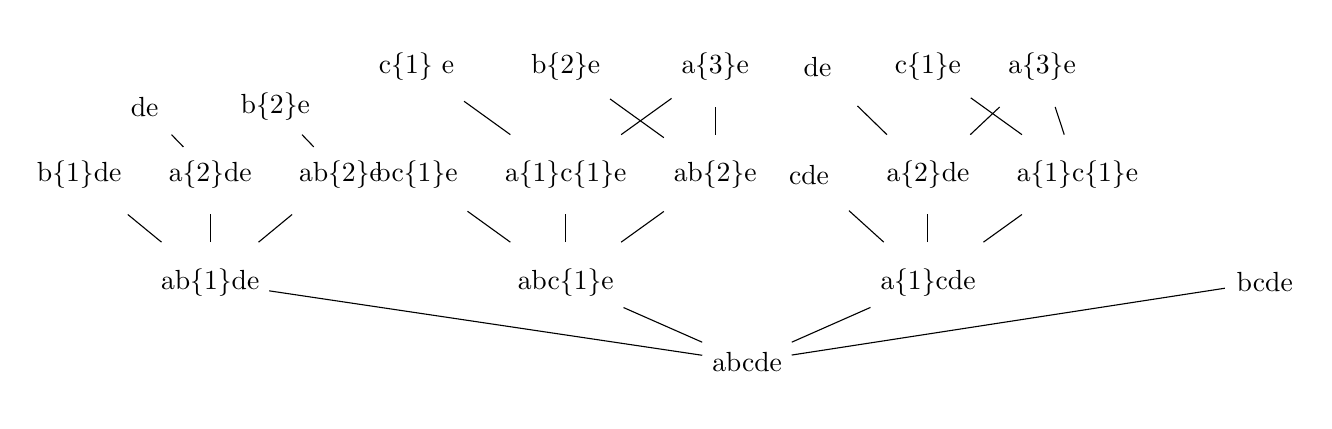
\begin{tikzpicture}[every node/.style={node distance=10pt, rectangle, minimum size=1cm}]
	\node[rectangle, minimum size=1cm](abcde) {abcde};
%     % I [above right=0.7cm and 4cm of A]
    \node[above left=0cm and 1cm of abcde](abcxe) {abc\{1\}e};
    \node[above=of abcxe](axcxe1) {a\{1\}c\{1\}e};
    \node[left=of axcxe1](bcxe1) {bc\{1\}e};
    \node[right=of axcxe1](abxxe1) {ab\{2\}e};
    \node[above=of bcxe1](cxe1) {c\{1\} e};
    \node[above=of axcxe1](bxxe1) {b\{2\}e};
    \node[above=of abxxe1](axxxe1) {a\{3\}e};
   %\draw (abxde) -> (bxde1);
    \draw (abcxe) -> (abxxe1);
    \draw (abcxe) -> (axcxe1);
    \draw (abcxe) -> (bcxe1);
    \draw (abxxe1) -> (axxxe1);
    \draw (axcxe1) -> (axxxe1);
    \draw (abxxe1) -> (bxxe1);
    \draw (axcxe1) -> (cxe1);
%     % II
    \node[above right=0cm and 1cm of abcde](axcde) {a\{1\}cde};
    \node[above=of axcde](axxde1) {a\{2\}de};
    \node[left=of axxde1](cde1) {cde};
    \node[right=of axxde1](axcxe2) {a\{1\}c\{1\}e};   
    \node[above=of axxde1](cxe2) {c\{1\}e};
    \node[left=of cxe2](de1) {de};
    \node[right=of cxe2](axxxe2) {a\{3\}e};
%    \draw (abxde) -> (bxde1);
    \draw (axcde) -> (axcxe2);
    \draw (axcde) -> (axxde1);
    \draw (axcde) -> (cde1);
    \draw (axcxe2) -> (axxxe2);
    \draw (axxde1) -> (axxxe2);
    \draw (axxde1) -> (de1);
    \draw (axcxe2) -> (cxe2);
    % III %% below
    \node[above left=0cm and 5.5cm of abcde](abxde) {ab\{1\}de};
    \node[above=of abxde](axxde2) {a\{2\}de};
    \node[left=of axxde2](bxde1) {b\{1\}de};
    \node[right=of axxde2](abxxe2) {ab\{2\}e};
    \node[above = of $(bxde1)!0.5!(axxde2)$](de2) {de};
    \node[above = of $(axxde2)!0.5!(abxxe2)$](bxxe2) {b\{2\}e};
    \draw (abxde) -> (bxde1);
    \draw (abxde) -> (axxde2);
    \draw (abxde) -> (abxxe2);
    \draw (axxde2) -> (de2);
    \draw (abxxe2) -> (bxxe2);
    % IV %% below
    \node[above right=0cm and 5.5cm of abcde](bcde) {bcde};
    %
    \draw (abcde) -> (abcxe);
    \draw (abcde) -> (bcde);
    \draw (abcde) -> (axcde);
    \draw (abcde) -> (abxde);
	\end{tikzpicture}
    \caption{Following the counts on  \cpageref{enum:minicorpus} we pruned the backoff graph from \cref{fig:bof}, which results in the backoff graph for \BOL. For each step the backoff procedure stops when it has occurred in the training data.}\label{fig:bol}
    \end{figure*}


In a setup with only $n$-gram features, \BON and \BOF are functionally the same in terms of backoff strategy. The nuance lies in the way they do the backoff. \BOF tries to backoff to skipgrams,\footnote{It tries, does not find the skipgram, since it is not trained on skipgrams, and continues with the backoff procedure.} independent of whether it was trained with skipgrams. The \BON strategy has only one way to get to the a-priori word probability. 
For \BOF it can get to the word probabilities for each skipgram that is generated, hence it puts more emphasis on the word probabilities.\footnote{Compare the number of paths to e in \cref{fig:bon} and \cref{fig:bof}.}

Now for the formal definition of the strategies, for all strategies, we have that $p(w|\mathbf{u})=G_0(w)$ if $\mathbf{u} = \emptyset$. For \BON, the other case is defined as:
  \begin{equation}\begin{split}
  	p(w|\mathbf{u})= &
\frac{c_{\mathbf{u}w\cdot}-d_{|\mathbf{u}|}t_{\mathbf{u}w\cdot}}{\theta_{|\mathbf{u}|}+c_{\mathbf{u}\cdot\cdot}} +
\frac{\theta_{|\mathbf{u}|}+d_{|\mathbf{u}|}t_{\mathbf{u}\cdot\cdot}}{\theta_{|\mathbf{u}|}+c_{\mathbf{u}\cdot\cdot}}
p(w|\pi(\mathbf{u}))
  \end{split}\end{equation}
%with $c_{\mathbf{u}wk}$ being the count of $w$ having the value $k$ after context $\mathbf{u}$; 
with $c_{\mathbf{u}w\cdot}$ being the number of $\mathbf{u}w$ tokens, and $c_{\mathbf{u}\cdot\cdot}$ the number of patterns starting with context $\mathbf{u}$. Similarly, $t_{\mathbf{u}wk}$ is 1 if the $k$th draw from $G_{\mathbf{u}}$ was $w$, 0 otherwise. $t_{\mathbf{u}w\cdot}$ then denotes if there is a pattern $\mathbf{u}w$, and $t_{\mathbf{u}\cdot\cdot}$ is the number of types following context $\mathbf{u}$.
  
Recall\footnote{See \cref{ch:languagemodels}.} that $\sigma_n$ is the operator that adds a skip to a pattern $\mathbf{u}$ on the $n$th position if there is not already a skip. Then $\boldsymbol\sigma(\mathbf{u}) = \left[\sigma_n(\mathbf{u})\right]_{n=2}^{|\mathbf{u}|}$ is the set of patterns with one skip more than the number of skips currently in $\mathbf{u}$. The number of generated patterns is $\boldsymbol\varsigma=|\boldsymbol\sigma(\mathbf{u})|$.
We also introduce the indicator function $S$, which for the {\sf full} backoff strategy always returns its argument: $S_{\mathbf{u}w}(y) = y$.
%
%
The {\sf full} backoff strategy is defined as follows, with $\mathbf{u}_x = \boldsymbol\sigma_x(\mathbf{u})$, and discount frequency $\delta_{\mathbf{u}} = 1$:
 \begin{equation}
 \begin{split}
p(w|\mathbf{u}) =& \sum_{m=1}^{\boldsymbol\varsigma}\left\{ \frac{1}{\mathbf{\boldsymbol\varsigma}+1}\left[
\frac{c_{\mathbf{u}_mw\cdot}-\delta_{\mathbf{u}_m}d_{|\mathbf{u}_m|}t_{\mathbf{u}_mw\cdot}}{\delta_{\mathbf{u}_m}\theta_{|\mathbf{u}_m|}+c_{\mathbf{u}_m\cdot\cdot}} + S_{\mathbf{u}_mw}\left(
\frac{\theta_{|\mathbf{u}_m|}+d_{|\mathbf{u}_m|}t_{\mathbf{u}_m\cdot\cdot}}{\delta_{\mathbf{u}_m}\theta_{|\mathbf{u}_m|}+c_{\mathbf{u}_m\cdot\cdot}}
p(w|\pi(\mathbf{u}_m))\right)\right] \right\} \\ 
+ 
%%
& \frac{1}{\mathbf{\boldsymbol\varsigma}+1}\left[
\frac{c_{\mathbf{u}w\cdot}-\delta_{\mathbf{u}}d_{|\mathbf{u}|}t_{\mathbf{u}w\cdot}}{\delta_{\mathbf{u}}\theta_{|\mathbf{u}|}+c_{\mathbf{u}\cdot\cdot}}+ S_{\mathbf{u}w}\left(\frac{\theta_{|\mathbf{u}|}+d_{|\mathbf{u}|}t_{\mathbf{u}\cdot\cdot}}{\delta_{\mathbf{u}}\theta_{|\mathbf{u}|}+c_{\mathbf{u}\cdot\cdot}}
p(w|\pi(\mathbf{u}))\right)\right]
  \end{split}\end{equation}
 
 The \BOL backoff strategy is an extension of the \BOF backoff strategy that stops the recursion if a test pattern $\mathbf{u}w$ has already occurred in the training data. This means that the count is not zero, and hence at training time a probability has been assigned to that pattern. $S$ is the indicator function which tells if a pattern has been seen during training: $S_{\mathbf{u}w}(\cdot) = 0$ if $\mathrm{count}(\mathbf{u}w) > 0$, $1$ otherwise; and $\delta_{\mathbf{u}} = V-\sum_{w\in W} S_{\mathbf{u}w}(\cdot)$. Setting $S_{\mathbf{u}w}(\cdot) = 0$ stops the recursion.

The backoff strategies \BON and \BOF always use the same number of backoff probabilities, for $5$-grams 5 and 53 respectively\footnote{For $4$-grams, 5 and 22 respectively.}. For \BOL this is dependent on the training material. If a top level pattern matches the training material, then only one probability is used. In the worst scenario, \BOL equals \BOF.

\section{Experimental Setup}

We train $4$-gram language models with the HPYPLM as described in this chapter, on three corpora as described in \cref{chap:data}. In this chapter we do not use sentences markers to denote the begin or end of a sentence. Since we do not compute the perplexity on sentence-level, but rather on individual patterns that comprise the test corpus.

At the core of our experimental framework we use \texttt{cpyp}\footnote{\url{https://github.com/redpony/cpyp}}, which is an existing library for non-parametric Bayesian modelling with Pitman-Yor priors with histogram-based sampling\autocite{blunsom2009note}. This library has an example application to showcase its performance with $n$-gram-based language modelling. Limitations of the library, such as not natively supporting skip- and flexgrams, and other functionality, such as thresholding and discarding of certain patterns, led us to extend the library with \texttt{Colibri Core}\footnote{\url{https://proycon.github.io/colibri-core/}}, a pattern modelling library. \texttt{Colibri Core} can handle these limitations\autocite{gompel2016efficient}, and together the libraries are a complete Bayesian language model that handles skipgrams.\footnote{The code and documentation is available at \url{https://github.com/naiaden/SLM}.}.

Each model is run for 50 iterations\footnote{Without an explicit burn-in phase, as we are not using statistics or samples from any but the last iteration.}, with hyperparameters $\theta = 1.0$, and $\gamma = 0.8$. The hyperparameters are resampled every 30 iterations\footnote{Which in practice results in one resampling of the hyperparameters.} with slice sampling\autocite{walker2007sampling}.

We test each model on different test sets, and we collect their intrinsic performance by means of perplexity. For the words in the test set that were unseen in the training data, we discard their probability.

\section{Results}
In this section we describe the results of multiple experiments. First we compare the HPYPLM approach to a traditional $n$-gram language model. We then show the influence of using skipgrams in addition to $n$-grams, and investigate whether this influence holds in a cross-domain evaluation. Second, we compare the backoff strategies, and investigate which domains fit which backoff strategy best.
\clearpage
\autocite{pickhardt2014generalized} report perplexity values on two subsets of the test material of jrc-p and wp-p\footnote{\textbf{Tell something about this!!}}. Of particular interest are the values for $n =4$, where for training on \wp and testing on wp-p a perplexity of 404 is reported with MKN smoothing, and 378 with their generalised language model (GLM). Similarly for the \jrc and jrc-p, they show a reduction of perplexity from 83 with MKN to 81 with their GLM. In our attempts to reproduce these values with SRILM\autocite{stolcke2002srilm}, we found substantially lower perplexity values for MKN,
\footnote{Lower perplexity values indicate a higher intrinsic performance, which is better.} as can be seen in \cref{tab:mknvsglm}.
\footnote{We used the following program call: \texttt{ngram-count -kndiscount -gt3min 1 -gt4min 1 -order 4 -interpolate -kndiscount -unk}.}
 The rows represent the train corpora; columns represent the test corpora. Comparing our results with the perplexity values reported for the GLM thus yields an unfair comparison. For this reason we choose the baseline to be the perplexity values from SRILM.

\begin{table*}
	\begin{tabular}{l*{6}{l}l*{6}{l}}
		&  \multicolumn{6}{c}{HPYLM} & &  \multicolumn{6}{c}{modified Kneser-Ney} \\
		& \jrc	& \obw	& \emea	&	\wp	& jrc-p	& wp-p & & \jrc	& \obw &	\emea & \wp&  jrc-p & wp-p\\ \cline{2-7}\cline{9-14}
		\jrc	& 13 & 1510 & 1081 & 1293 & 13 & 1269 & & 22 & 1664 & 1310 & 1837 & 122 & 1736 \\
		\obw & 1232 & 171 & 1749 & 724 & 1156 & 692 & & 1460 & 211 & 1516 & 996 & 1383 & 1046 \\
		\emea & 769 & 1552 & 4 & 1097 & 774 & 1093 & & 1115 & 1745 & 10 &1669 & 993 & 1444 \\
		wps & 555 & 455 & 1005 & 217 & 537 & 212 & & 842 & 598 & 1590 & 449 & 1088 & 646
	\end{tabular}
	\caption{A side-by-side comparison of perplexities of two $n$-gram language models with $n=4$: the Bayesian hierarchical Pitman-Yor language model (HPYLM) and the frequentist modified Kneser-Ney, as implemented by SRILM. The rows represent the training corpora, and the columns the test sets. }\label{tab:mknvsglm}
		%The two additional data sets jrc-p and wp-p are around 100k randomly selected 4-grams from jrc and wp respectively, as selected by \newcite{pickhardt2014generalized}. 
\end{table*}

\autocite{teh2006hierarchical} shows that the HPYPLM can outperform MKN. In our experiments we reach the same conclusion, on the basis of the results listed in \cref{tab:mknvsglm}. On the right we show the results with SRILM's implementation of MKN, now without sentence boundaries, equal to the settings of our HPYPLM. The perplexities obtained by the HPYPLM are consistently lower by a substantial margin.

Bayesian language models are more complex than their frequentist counterparts such as MKN. Not only the model itself is more complex, but also the computational complexity, both in terms of time and memory. On an Intel Xeon E5-2660 with 512G working memory it takes 3 days to compute the \obw model, and serialize the model to file. However, if we only use one iteration for sampling,\footnote{With zero sampling iterations, we have effectively reduced the HPYPLM to IKN.} we already achieve perplexities approaching the perplexities reported in \cref{tab:mknvsglm} with 50 iterations, in all setups. This one-iteration learning process does not alleviate the burden of memory complexity\footnote{The number of parameters only changes when a restaurant has no visitors, or when one is being founded. The number of customers stays constant over all sampling iterations.}, but training is now only a factor two slower than traditional MKN, and the performance is already notably better.
Yet, in the remainder of this chapter we use 50 iterations for Gibbs sampling. For testing, once the model has been loaded into memory, there is no time penalty involved when choosing HPYPLM over MKN, which is an important property for extrinsic and time-dependent evaluation.

\subsection{Influence of adding skipgrams to an $n$-gram language model}
The results for English language models with skipgrams are reported in \cref{ta:ngramvsskipgram} in terms of perplexity. The rows represent the train corpora, and columns the test corpora. On the diagonals the perplexity always has the lowest value for that column, since the best performance on a test set is achieved by training on the same domain, for all domains. 

We also observe an effect of domain-specific versus generic corpora. The within-domain performance of domain-specific corpora yields very low perplexities (13 on \jrc, 4 on \emea), while these are higher for within-domain evaluation for generic corpora (158 for \obw, 216 for \wp). There is no difference between training with only $n$-grams and training with skipgrams on within-domain test sets.

     \begin{table*}
	\begin{tabular}{lllllllllllllll}
		& \multicolumn{4}{c}{$n$-grams}	& & \multicolumn{4}{c}{skipgrams}&& \multicolumn{4}{c}{Relative difference (in \%)}\\
		& \jrc	& \obw	& \emea	& \wp	& & \jrc	& \obw	& \emea	& \wp	& & \jrc	& \obw	& \emea	& \wp \\ \cline{2-5}\cline{7-10} \cline{12-15}
		\jrc		& 13	& 1195	& 961	& 1011	& & 13	& 1162	& 939	& 1008	& & 0	& -3	& -2	& 0		\\
		\obw	& 1232	& 171	& 1749	& 724	& & 728	& 141	& 1069	& 542	& & -41	& -6	& -39	& -25	\\
		\emea	& 600	& 1143	& 4		& 843	& & 581	& 1155	& 4		& 842	& & -3	& 1	& 1		& 0		\\
		wps		& 555	& 455	& 1005	& 217	& & 565	& 470	& 990	& 227	& & 2	& 3	& -1	& 4
	\end{tabular} 
	\caption{An overview of the results to compare the influence and contribution of skipgrams for English. 
		The perplexities can only be compared row-wise, as the vocabulary depends on the training set. For these values we chose the best-performing backoff strategy. The relative difference is the percentual change, with a negative value indicating an improvement with skipgrams.}\label{ta:ngramvsskipgram}
\end{table*} 

However, we find that adding skipgrams does tend to contribute to a lower perplexity in a cross-domain setting, with many non-diagonal cells showing lower perplexities. We observe absolute perplexity reductions up to 33, and relative reductions up to 3.2\%. We are mostly interested in the effects of training on a generic corpus, and testing on a domain-specific corpus: it is generally easier to obtain generic texts, and even if there is a corpus for that specific domain, there will always be more generic data. If it turns out that the generic corpora can be used to model domain-specific corpora without much deterioration, this paves the way to fully use the billion-word data sets that are currently available for many languages.\footnote{COW CORPUS} If we focus on the rows for \obw and \wp, we see that for the cross-domain setups with \jrc and \emea, the performance improves when we add skipgrams to the input features, except when we test \jrc trained on \wp.

In particular we focus on \obw for the remainder of this thesis, since compared to \wp, which contains articles in Wikipedia's encyclopaedic style, it contains a wider variety of text, and is less restricted in language use. Supported by the perplexity results, we consider \wp to be less generic.\footnote{This is independent of the number of words.} This is reflected in the perplexity scores as well, where a within-domain experiment on \wp (227 ppl) appears to be more difficult than on \obw (141 ppl). In the \obw-\wp and \wp-\obw experiments the perplexities are more in range, 542 and 470 respectively.

\subsection{Effect of different backoff methods}
In the previous subsection we compared pure $n$-gram models with skipgram models, where we used the best performing backoff methods. In this subsection we study the effect of different backoff methods in more detail. 

Although skipgram models also contain all $n$-grams as an $n$-gram model trained on the same data, the $n$-gram probabilities differ between the two models. If we train with skipgram features, but only use the $n$-gram during testing (\BON), one would expect the same perplexity. However, a side-effect of training with skipgrams is that the lower-order patterns contained in the skipgrams are seen more often, compared to training with only $n$-grams.

In our analyses we included this strategy to see the negative effects of using skipgrams, because even in scenarios where they do not contribute, \BON may still yield a perplexity similar to HPYPLM trained on only $n$-grams. If that is the case, we can opt to use skipgrams whenever possible, without risking a deterioration in performance.

The \BOF backoff strategy is effective especially in cross-domain situations, where backing off to the word probabilities is beneficial. We see this especially in \jrc and \emea; for \wp this effect is not present. If we compare the OOV rate for \wp on cross-domain sets, it is consistently higher than the OOV rate for \obw on other sets. This explains why a backoff procedure which emphasises the word level more does not help in such cases.

For a within-domain experiment on \obw, we notice that throughout the learning curve until 30M words, \BOF is slightly outperforming \BOL. But with more training data, \BOL has seen enough $n$-grams to overtake \BOF.

\subsection{Observations from \obw learning curves}

The learning curves for \obw are shown in \cref{fig:1bwlc}. The pure $n$-gram models are outperformed by the skipgram models, for all four test sets. We are mostly interested in comparing \BON with the best performing skipgram backoff method.

The first observation is that the skipgrams are especially useful in the beginning, when the perplexity is very low. However, we have to `discard' these values, since at this point there are still too many OOV words and therefore it models only few words. Only after the learning curve drops, we consider the values to be of use. Here the perplexity of the skipgram models is consistently lower than those of \BON. Since the \BON models have a higher peak in the learning curve, it is also easier to gain a reduction in perplexity with an increasing number of training words. But with the amount of training data we have the models do not converge for cross-domain testing. For none of the eight models plotted in \cref{fig:1bwlc} we see any plateauing behaviour, indicating that all eight models gain from having (yet even) more train data.

In the same plot we can also see that there is a clear distinction between the test sets. The behaviour of testing on \obw, is different compared to testing on \jrc, \emea, or \wp. They share the same progression, with \wp's course shifted downwards\footnote{Since it shares the same property of being more generic than \jrc and \emea.}, unlike the domain-specific sets. \BON and \BOF of these models also seem to have a gap, whereas \BON and \BOL of \obw are converging at the end. This seems to confirm that skipgrams are especially useful in cross-domain settings, where with order of magnitude more data, the lines do not seem to converge.\footnote{Although we do not have in fact more data, we extrapolated this bevahiour on the basis of the plots.}

For within-domain we have reached a point where we have seen enough $n$-grams to estimate the probabilities, and the patterns modelled by skipgrams are also covered sufficiently by $n$-grams. We verified this by checking to which level the models backoff, and find that with an increasing amount of training material, the average backoff depth is smaller, and that for out-of-domain experiments the average backoff depth is larger.

\begin{figure*}
	\begin{tikzpicture}
	\begin{axis}[
	height=6cm, width=8cm, legend cell align=left, legend style={legend pos=north west, fill=none, font=\small},
	title=Testing on general texts,
	xmode = log,
	xmin=800,xmax=2048576000,
	%ymin=-100,ymax=40,
	xlabel=Train corpus size (\obw; in words),
	ylabel=Perplexity]
	\addplot[brown,thick] table [x=1bw, y=ngram]{data/1bw-1bw.dat};
	\addlegendentry{\obw \BON}
	\addplot[brown,thick,dotted] table [x=1bw, y=limited]{data/1bw-1bw.dat};
	\addlegendentry{\obw \BOL}
	%\addplot[brown,thick,dashed] table [x=1bw, y=full]{1bw-1bw.dat};
	%\addlegendentry{1bw full}
	\addplot[black,thick] table [x=wp, y=ngram]{data/1bw-wp.dat};
	\addlegendentry{\wp \BON}
	\addplot[black,thick,dashed] table [x=wp, y=full,mark=*]{data/1bw-wp.dat};
	\addlegendentry{\wp \BOF}
	\end{axis}
	\begin{axis}[
	height=6cm, width=8cm, legend cell align=left, legend style={legend pos=north west, fill=none, font=\small},
	title=Testing on domain-specific texts,
	xmode = log,
	xmin=800,xmax=2048576000,
	%ymin=-100,ymax=40,
	xlabel=Train corpus size (\obw; in words),
	xshift=8cm]
	\addplot[blue,thick] table [x=jrc, y=ngram]{data/1bw-jrc.dat};
	\addlegendentry{\jrc \BON}
	\addplot[blue,thick,dashed] table [x=jrc, y=full]{data/1bw-jrc.dat};
	\addlegendentry{\jrc \BOF}
	\addplot[red,thick] table [x=emea, y=ngram]{data/1bw-emea.dat};
	\addlegendentry{\emea \BON}
	\addplot[red,thick, dashed] table [x=emea, y=full,mark=*]{data/1bw-emea.dat};
	\addlegendentry{\emea \BOF}
	\end{axis}
	\end{tikzpicture}
	\caption{Learning curve for training on \obw, and testing on \obw and \wp on the left, and \jrc and \emea on the right. The solid lines indicate the perplexity of the \BON model, the dotted line \BOL for testing on \obw, and the dashed lines \BOF for \jrc, \emea, and \wp.}\label{fig:1bwlc}
\end{figure*}

 \section{Behaviour of the Language Models}
Aside from a quantitative analysis in terms of perplexity, we are also interested in the qualitative differences between the compared approaches. In this section we analyse the skipgrams that contribute the most, and which are most prominent. We finish the section with a look at the models from a Zipfian point of view, and compare the frequentist and Bayesian rank-ordered frequencies.

\subsection{When do skipgrams work?}
Earlier we stated that skipgrams can be part of the solution for modelling long-range dependencies and shorter-range non-contiguous patterns. In the experiments described in this paper we have limited ourselves to modelling each skip with one token, where skips must be surrounded by word tokens. This limits the skipgrams of length $4$ as used in this paper to at most two position skips.

To understand which patterns can be modelled with these skipgrams, and in particular, which of these patterns contribute positively to a better score, we analysed all $4$-grams in the test data which have a higher posterior probability with skipgram features added to the training model. 
%
To this end, we analysed the results of one run in which we trained on \obw and tested on the 2.2M $4$-grams in \emea. Of those $4$-grams 473 thousand showed a lower perplexity when adding skipgram features, as compared to the standard $n$-gram model. 

In this section we approach the question from three different angles. First we consider the skipgrams patterns boost probability of test patterns. Second, we look at the most-frequent skipgram patterns that cause a lower perplexity for the skipgram model. Third, we are interested in the patterns with high-frequent words that skip over low-frequent words, because they are not only frequent themselves, but also invariant to domains. 


\begin{table*}
	\small
	\begin{tabular}{lllllll}
		most helpful  & & most-frequently helpful & & skip on second & & skip on third \\ \cline{1-1}\cline{3-3}\cline{5-5}\cline{7-7}
		if the \{1\} blood & & , \{2\} , & & the \{1\} of the &  & in the \{1\} of\\
		: in \{1\} with & & ( \{2\} ) & & the \{1\} of a   & & to the \{1\} of\\
		treatment \{1\} cervical cancer   & & see \{2\} ) & & , \{1\} , and    & & on the \{1\} of\\
		product \{1\} due to & & see section \{1\} ) & & The \{1\} of the & & of the \{1\} of\\
		result \{1\} due to & & of \{2\} and & & and \{1\} of the & & of the \{1\} . \\
	\end{tabular}
	\caption{First column contains the 5 most-helpful patterns; the second column the 5 most-frequently helpful patterns. The third and fourth column contain the top-5 most-frequent skipgrams with their frequency, with the skip on the second (left) and third (right) position, when the skipped word is 20 or more times less frequent than the least frequent word in the skipgram.}\label{ta:examples}
\end{table*}


%(': {1} accordance with', 0.15049816926667361),
% (': in {1} with', 0.15049816926667361),
% ('treatment {1} cervical cancer', 0.10562404017518799),
% ('product {1} due to', 0.09975897235968394),
% ('result {1} due to', 0.07797193841653396),


Patterns with the largest difference in probability are typically domain-specific patterns of which the words occur in the training data, but where there is no direct $n$-gram match. See \cref{ta:examples} for 5 examples. 
%The pattern \emph{such as myocardial infarction} is a very domain-specific pattern, and as such does not occur in 1bw. However, since parts of it occurs in multiple forms (\emph{bowel infarction}, \emph{celebral infarction}, etc.), having a skipgram \emph{such as \{1\} infarction} is beneficial.
%The pattern \emph{intestines ( ulcerative colitis} is a very domain-specific pattern, and as such does not occur in 1bw. However the trigram \emph{( ulcerative colitis} occurs once, and its bi-, and unigram \emph{ulcerative colitis} and \emph{colitis} occur 189 and 337 times. We showed earlier that adding skipgrams add causes the subpatterns in the skipgrams to be added: e.g. each bigram is added twice. Additionally \emph{full} places an emphasis in the backoff procedure on the unigrams, which helps improving the probability of this pattern a lot.
The pattern \emph{if the systolic blood} is a very domain-specific pattern in \emea, and is not covered by \obw. However, the pattern \emph{if the \{1\} blood} occurs in multiple forms (e.g.\ \emph{bad blood}, \emph{maternal blood}, \emph{' blood}). Although there is match for \emph{the systolic blood} in \obw, the skipgrams help to boost the probability with over $0.15$. 
%An example is \emph{: in accordance with}, whose high-frequency is also domain-specific for biomedical texts (326 times in emea). The improvement of the probability is not caused by emphasising the unigrams, but because of the skipgram patterns added. As a whole it occurs once in 1bw. The skipgram \emph{: \{2\} with} occurs 3969 times, \emph{: \{1\} accordance with} and \emph{: in \{1\} with} 6 and 22 times respectively. Leaving out the first marker gives an even better clue: 1bw contains 143909 occurrences of \emph{in \{1\} with} .

On the other hand, the patterns with the largest difference in probability only occur very sparsely. To explain the gain in perplexity when adding skipgrams, we have to look at patterns with a lower probability that occur often. Here we see that these patterns are less domain-specific.
%
%The first example \emph{e . g .} seems odd, but in the training data only \emph{e , g .} occurs, hence the skipgram is able to give a better estimation. Since this example occurs 1346 times, this has the potential to make a huge difference in the final perplexity.

The texts in \emea contain many subordinate clauses and parenthesised phrases, for clarification. Since \obw is a different domain, we do not find these clauses and phrases verbatim in the train data. However, we do find patterns such as \emph{, \{2\} ,} and \emph{( \{2\} )} a lot. Knowing that a lot of clauses and phrases are of length 2, these skipgrams contribute a little each time an opening parenthesis occurs, when the focus word is a closing parenthesis. The improvement is subtle, but accumulated over all test patterns, this amounts for a noticeable change in the perplexity.

%The patterns above are mostly composed out of content words. For the last analysis we look at patterns composed of function words. 
From the 473 thousand patterns that obtained a lower perplexity we first discarded specific patterns through imposing an occurrence ratio threshold of 20 on the words in the skips. This means that if the skip is $\{1\}$, that word must occur at most 20 times less often than the least frequent of the three other words, and in case of $\{2\}$ the two words must occur at most 20 times less than the least frequent of the other two words. This ratio models the suspicion that skipgrams are particularly useful in situations where the skip models a low-frequent content word. 

We hardly observe any other patterns than these function-word patterns. 
This may be caused by the fact that \emea is very domain-specific, and that matches on content words are unlikely to occur often. It may be precisely because of this feature of \emea that the skipgrams, extracted from \obw, are providing the kind of effective modelling of non-contiguous patterns to be able to skip unknown words and continue matching with (function) words further to the left.

In the analysis we listed all 473k $n$-grams, and artificially added skips in the three possible manners, e.g.~\emph{in the previous section} has as three possible skipgrams \emph{in \{1\} previous section} (1), \emph{in the \{1\} section} (2), and \emph{in \{2\} section} (1,2). We then put occurrence ratio thresholds (20, 10, 5) on the words in the skips. For ratio 20 this means that if the skip is \{1\} that word must occur at most 20 times less than the least frequent of the three other words, and in case of \{2\} the two words must occur at most 20 times less than the least frequent of the other two words. This ratio models the suspicion that skipgrams are particularly useful in situations where the skip models a low-frequent word. 

\begin{table*}
	\begin{center}
		\begin{tabular}{l*{3}{l}l*{3}{l}l*{3}{l}}
			& \multicolumn{3}{c}{5} & & \multicolumn{3}{c}{10} & & \multicolumn{3}{c}{20} \\
			& \obw & tokens & types & & \obw & tokens & types & & \obw & tokens & types \\
			\cline{2-4}\cline{6-8}\cline{10-12}
			1 & 7.5M & 3.6k & 1.9k & & 5.8M & 2.9k & 1.4k & & 4.4M & 2.2k & 1.0k \\
			2 & 7.6M & 5.2k & 3.6k & & 5.9M & 4.2k & 2.1k & & 4.4M & 3.3k & 1.5k \\
			1,2 & 5.2M & 2.9k & 526 & & 4.2M & 2.3k & 362 & & 3.3M & 1.8k & 258 \\
		\end{tabular}
		\caption{The number of patterns with skipped-word-ratio respectively in \obw, the number of skipgram token matches with the \emea test set, and the skipgram types that match with the frequency ratio filtered skipgrams. The rows denote the position of the skip (starting with index $0$), and the columns indicate the ratio in which the words in the skip must occur with respect to their surrounding words. This table shows that there are only few patterns that benefit from adding skipgrams.}\label{ta:skipratio}
	\end{center}
\end{table*}

In the last phase we count all the skipgram types generated from the four-grams that yielded a lower perplexity when adding skipgram features. \Cref{ta:skipratio} lists the occurrence counts of skipgram tokens and types for the \obw-\emea experiment where we varied the frequency ratio in which the skipped words must occur with respect to their surrounding words. It becomes apparent that only a limited number of patterns benefit from adding skipgrams as features.

As an illustration we list in the last two columns of \cref{ta:examples} the five most frequent skipgrams types with the skip on position 2 and with occurrence ratio 20, and with a skip on position 3.

%	If we look at which patterns are predicted better, and if we drop the concept of frequency ratio in skipgrams, then different patterns do emerge. For example, in the training data there is only one mention of `Merck Sharp \& Dohme'. Being a pharmaceutical company, there are many mentions in the test data (emea), but in more variations, such as: `Merck Sharp \& Dohme', `Merck Sharp and Dohme', `Merck Sharp E Dohme'. The pattern that attains a lower perplexity skips the third word. This is a case where skipgrams help with patterns that are not composed of function words.

Another type of effective pattern is one that skips over a numerical value. Medical prescriptions often contain mentions of quantities or concentrations, for example expressed by ``with consideration for the haemoglobin target range of 10 g / dL ( 6.2 mmol / l )''. Skipgrams are particularly useful in skipping over the number positions, as the patterns surrounding them are fixed and frequent. This step is often implicit in language modelling, when all numbers are mapped to a special token, i.e.\ \{\#\#\#\}. With skipgrams, the numerical value can be preserved.


\begin{figure*}
	\centering
	\begin{tikzpicture}
	\begin{loglogaxis} [
	width=5cm,
	height=3cm,
	scale only axis,
	enlargelimits=false,
	axis on top,
	xlabel=Rank,
	ylabel=Frequency,
	title=$n$-grams,
	ylabel shift=-0.1cm, legend cell align=left, legend style={only marks, legend pos=north east
		, font=\small}
	]
	\addplot+ graphics [ 
	xmin=1,
	xmax=4746593,
	ymin=1,
	ymax=369489,
	] {figures/n1.png};
	
	\end{loglogaxis}
	\begin{loglogaxis} [
	width=5cm,
	height=3cm,
	scale only axis,     
	enlargelimits=false,   
	axis on top,        
	xlabel=Rank,
	title=$n$-grams and skipgrams,
	xshift=7cm, legend cell align=left, legend style={at={(8cm,3cm)}
		, only marks
		, font=\small}
	]
	\addplot+ graphics [
	xmin=1,
	xmax=7370640,
	ymin=1,
	ymax=4014991,
	] {figures/s1.png};
	\addlegendimage{only marks, black, mark=*}
	\addlegendentry{\obw train}
	\addlegendentry{\obw HPYPLM}
	\addlegendentry{\jrc test}
	\addlegendentry{\obw test}
	\addlegendimage{only marks, red, mark=*} % or mark=none?
	\addlegendimage{only marks, brown, mark=*}
	\addlegendimage{only marks, blue, mark=*}
	
	\end{loglogaxis}
	\end{tikzpicture}
	\caption{Log-log frequency-rank curves 
		and scatter plots for three sets, the complete \obw (train and test), and the deviating estimated frequencies of the HPYPLM (black). The ranks are determined on the heldout data.
		}\label{fig:freqs}
\end{figure*}

\subsection{An analysis of the $n$-gram distribution}
Because the HPYPLM is a Bayesian generalisation of the IKN language model, and in some circumstances also to MKN, we are interested in the differences between the two methods. 
%     %In this subsection we analyze the word distributions, for the complete corpus, the trainings data, and the posterior trigram distribution for the HPYLM.

We know that words and word $n$-grams in a language manifest themselves typically in power-law distributions. Few patterns occur very often, whereas the majority of patterns are only observed very sparsely. For this reason we chose the HPYPLM, as the Pitman-Yor prior can model this power-law behaviour. The power-law growth of patterns in language has been popularized by the early work of George Zipf \autocite{Zipf35,Zipf49}. Recently, \autocite{piantadosi2014Zipfs} has asserted that most Zipfian analyses have been done under false premises, namely that the frequency of the words is determined on the same data set as which is used to determine the rank of the words. In this subsection we analyse the rank of the patterns on the heldout set of \obw, and determine the frequency on the training sets. The trigrams in the remainder of this section are context trigrams, the part of fourgrams before the focus word.

In \cref{fig:freqs} we plot the frequency for each trigram in the heldout set of \obw. The brown dots
follow a typical Zipfian curve since the rank is determined on the same set. The blue dots are the frequencies of the trigrams in the complete \obw, ordered by the rank as found on the heldout data. Invisible in the scatter plot, there are patterns that occur in the training data but not in the heldout data (since the heldout data was unseen data).
The blue dots also represent the frequencies as used by MKN, which does not manipulate the data by changing the word counts. The black dots are the frequencies as estimated by the HPYPLM. 

In general we observe that most deviating frequency estimations are in the tail, where we can find many patterns that do not occur in the heldout data, but have a positive frequency in the training data. Trigram tokens are mostly re-distributed by HPYPLM among those patterns.\footnote{A sum of all frequencies confirms that tokens are not lost in the process.}

If we train with only $n$-grams, HPYPLM follows the counted frequencies, but as the rank increases, the effect of sampling and re-estimating frequencies by the HPYPLM is quite apparent (the black points not shadowed by the blue cloud). For the high frequency data the frequencies are estimated lower, whereas the remainder of the counts is used to boost the patterns that have a lower rank. If we add skipgram features, than HPYPLM's cloud is more spread-out, and its power-law behaviour is less explicit. Here also we see that the counts of higher-ranked patterns are diminished to boost lower-ranked patterns.

Another observation we make is that if we train on \obw, yielding the distributions as shown in \cref{fig:freqs}, and we test on a specific domain such as \jrc (the red dots in the figure), we see that if we only train on $n$-grams, the dots are quite dispersed into a cloud, and that this distribution over frequencies differs substantially from the distributions from \obw. For the skipgram-trained model we see that the red dots are less dispersed, somewhat more closely following a Zipfian distribution, with a decay similar to the training points for the HPYPLM estimated frequencies of \obw.

\subsection{Variation in HYPLMs}
In this subsection we briefly show an analysis of the variability of the perplexity of the HPYLM approach, both in terms of iterations used for sampling, and in terms of stability over multiple runs. These analyses support the idea that the reductions in perplexity mentioned earlier in this paper are not due to some random effect, by choosing a favourable `best' run, or halting at an specific or large number of iterations.


%     One of the major concerns of Bayesian models are their intractability. To avoid these complications, clever inference schemes have been proposed. In our methods we use Gibbs sampling for the seating arrangement, and slice sampling for the hyperparameters. Still, each new run leads to a different outcome. 

\begin{figure*}
	\begin{tikzpicture}
	\begin{axis} [
	%width=0.25\textwidth,
	height=4cm,
	scale only axis,        % Plot size does not include axes.
	enlargelimits=false,    % Shrink wrap the PNG.
	axis on top,            % Axes placed over PNG to avoid obscuring the lines.
	xlabel=Iterations,
	ylabel=Perplexity,
	]
	\addplot graphics [
	xmin=1,
	xmax=150,
	ymin=1181.23,
	ymax=1192.63,
	] {figures/jrc1bwglm.pdf};
	\end{axis}
	%     \begin{axis} [
	%     	width=0.25\textwidth,
	%         scale only axis,        % Plot size does not include axes.
	%         enlargelimits=false,    % Shrink wrap the PNG.
	%         axis on top,            % Axes placed over PNG to avoid obscuring the lines.
	%         xlabel=Iterations,
	%         xshift=0.33\textwidth
	%     ]
	%         \addplot graphics [
	%             xmin=1,
	%             xmax=150,
	%             ymin=61.6039,
	%             ymax=66.3028,
	%         ] {jrcjrcglm.pdf};
	%     \end{axis}
	\begin{axis} [
	%width=0.25\textwidth,
	height=4cm,
	scale only axis,        % Plot size does not include axes.
	enlargelimits=false,    % Shrink wrap the PNG.
	axis on top,            % Axes placed over PNG to avoid obscuring the lines.
	xlabel=Iterations,
	xshift=8cm
	]
	\addplot graphics [
	xmin=1,
	xmax=150,
	ymin=13.2062,
	ymax=13.3504,
	] {figures/jrcjrcngram.pdf};
	\end{axis}
\end{tikzpicture}
\caption{Variation over 10 runs. On the left is \jrc-\obw-\BOF, on the right is \jrc-\jrc-\BON. The red lines show the perplexity values for one of the 10 runs, and the blue lines show the min and max values per iteration over the 10 runs.}\label{fig:iterplots}
\end{figure*}


We evaluate on the test sets \jrc and \obw, trained on $n$-grams and skipgrams, with backoff strategies \BON and \BOF, in ten individual runs with up to 150 iterations each, with the same training data. We measure perplexity on the respective test sets at every iteration. We find that there are only minor differences in perplexities between runs (maximal and minimal values denoted by the blue lines) with respect to the average over the 10 runs (the red line). This is the case in high-perplexity scenarios such as \jrc-\obw-\BOF, with perplexities around 1184, and low-perplexity scenarios such as \jrc-\jrc-\BOF with perplexities around 13.2. The perplexities also converge quickly, within 50 iterations.
\footnote{Although we do not take burn-in and autocorrelation between iterations into consideration.}

\section{Discussion}
In this paper we showed that by adding skipgrams, a simple generalisation of $n$-gram word patterns, we can reduce the perplexity of a Bayesian language model in a cross-domain language modelling task. The model, a Hierarchical Pitman-Yor Process Language Model (HPYPLM) was observed to attain lower perplexities than the standard modified Kneser-Ney smoothing $n$-gram language model in all training-test conditions, confirming results reported in earlier work \autocite{teh2006hierarchical}.

Although the extension of HPYPLM to skipgrams is relatively easy to implement, it has a considerable impact on the complexity. Since the number of patterns almost doubles, so does the run-time of the learning phase. Compared to the modified Kneser-Ney implementation of SRILM, training the HPYPLM is markedly slower. However, within a single iteration of sampling the approach already improves over modified Kneser-Ney. If one would halt here, runtime complexity is reduced to a factor two compared to modified Kneser-Ney with SRILM. The improvements of our HPYPLM variant over the SRILM (and most other) modified Kneser-Ney implementations is that it can handle skipgrams in their full form. The testing phase of either methods is comparable in terms of computational complexity, which puts the HPYLM in a preferable position.
%\chapter{Domain-adaptation with a double hierarchical Pitman-Yor skipgram language model}

\part{Extrinsic evaluation}
%\chapter{Chapter 4\newline The influence of skipgrams on automatic speech recognition}\label{ch:speech}
%\chapter{Relating brain activity data to perplexities from skipgram models}
%\chapter{Using skipgram language models in automatic speech recognition for under-resourced languages}

\chapter{Conclusion}

%\chapter{Derivation and proof for the hierarchical Pitman-Yor process language model with added interpolation factors and backoff strategies}\label{apx:proofinterpolform}

In the original paper by Teh,\autocite{teh2006hierarchical} the functions\footnote{Ibidem, Equations 10 and 11.} that return the word probability are defined as:

\begin{equation}
\begin{split}
p(w | 0, \mathcal{S}, \Theta) =& 1/V \\
p(w | \mathbf{u}, \mathcal{S}, \Theta) =& \frac{c_{\mathbf{u}w\cdot} - d_{|\mathbf{u}|}t_{\mathbf{u}w\cdot}}{\theta_{|\mathbf{u}|}+c_{\mathbf{u}\cdot\cdot}} + \frac{\theta_{|\mathbf{u}|} + d_{|\mathbf{u}|}t_{\mathbf{u}\cdot\cdot}}{\theta_{|\mathbf{u}|}+c_{\mathbf{u}\cdot\cdot}} p(w | \pi(\mathbf{u}), \mathcal{S}, \Theta)
\end{split}
\end{equation}

Since these formulae will serve as the basis for our \textsl{limited} backoff strategy, we show its correctness. A step we also have to show for our derivation.

We show its correctness by showing that the probability distribution sums up to one (and that it is not negative, and the elements are not bigger than 1).

Assume there is a dictionary $W$ with $V$ words. Then we can sum over all customers in each restaurant, for all dishes with $\sum_{w\in W} c_{\mathbf{u}w} = c_{\mathbf{u}\cdot\cdot}$, and similarly for the tables: $\sum_{w\in W} t_{\mathbf{u}w\cdot} = t_{\mathbf{u}\cdot\cdot}$. 
\begin{equation}
\begin{split}
	\sum_{w\in W} p(w | \mathbf{u}, \mathcal{S}, \Theta) = 1 \\
    \sum_{w\in W}\frac{c_{\mathbf{u}w\cdot} - d_{|\mathbf{u}|}t_{\mathbf{u}w\cdot}}{\theta_{|\mathbf{u}|}+c_{\mathbf{u}\cdot\cdot}} + \frac{\theta_{|\mathbf{u}|} + d_{|\mathbf{u}|}t_{\mathbf{u}\cdot\cdot}}{\theta_{|\mathbf{u}|}+c_{\mathbf{u}\cdot\cdot}} p(w | \pi(\mathbf{u}), \mathcal{S}, \Theta) = 1 \\
    \sum_{w\in W}\frac{c_{\mathbf{u}w\cdot} - d_{|\mathbf{u}|}t_{\mathbf{u}w\cdot}}{\theta_{|\mathbf{u}|}+c_{\mathbf{u}\cdot\cdot}} + \sum_{w\in W} \frac{\theta_{|\mathbf{u}|} + d_{|\mathbf{u}|}t_{\mathbf{u}\cdot\cdot}}{\theta_{|\mathbf{u}|}+c_{\mathbf{u}\cdot\cdot}} p(w | \pi(\mathbf{u}), \mathcal{S}, \Theta) =1 \\
    \sum_{w\in W} \frac{c_{\mathbf{u}w\cdot}}{\theta_{|\mathbf{u}|}+c_{\mathbf{u}\cdot\cdot}} - \sum_{w\in W} \frac{d_{|\mathbf{u}|}t_{\mathbf{u}w\cdot}}{\theta_{|\mathbf{u}|}+c_{\mathbf{u}\cdot\cdot}} + \sum_{w\in W} \frac{\theta_{|\mathbf{u}|}p(w | \pi(\mathbf{u}), \mathcal{S}, \Theta)}{\theta_{|\mathbf{u}|}+c_{\mathbf{u}\cdot\cdot}} + \sum_{w\in W} \frac{d_{|\mathbf{u}|}t_{\mathbf{u}\cdot\cdot} p(w | \pi(\mathbf{u}), \mathcal{S}, \Theta)}{\theta_{|\mathbf{u}|}+c_{\mathbf{u}\cdot\cdot}} = 1 \\
    \frac{c_{\mathbf{u}\cdot\cdot}}{\theta_{|\mathbf{u}|}+c_{\mathbf{u}\cdot\cdot}} - \frac{d_{|\mathbf{u}|}t_{\mathbf{u}\cdot\cdot}}{\theta_{|\mathbf{u}|}+c_{\mathbf{u}\cdot\cdot}} + \theta_{|\mathbf{u}|}\sum_{w\in W} \frac{p(w | \pi(\mathbf{u}), \mathcal{S}, \Theta)}{\theta_{|\mathbf{u}|}+c_{\mathbf{u}\cdot\cdot}} + d_{|\mathbf{u}|}t_{\mathbf{u}\cdot\cdot}\sum_{w\in W} \frac{ p(w | \pi(\mathbf{u}), \mathcal{S}, \Theta)}{\theta_{|\mathbf{u}|}+c_{\mathbf{u}\cdot\cdot}} = 1 \\
    \frac{c_{\mathbf{u}\cdot\cdot}}{\theta_{|\mathbf{u}|}+c_{\mathbf{u}\cdot\cdot}} - \frac{d_{|\mathbf{u}|}t_{\mathbf{u}\cdot\cdot}}{\theta_{|\mathbf{u}|}+c_{\mathbf{u}\cdot\cdot}} +\frac{ \theta_{|\mathbf{u}|}}{\theta_{|\mathbf{u}|}+c_{\mathbf{u}\cdot\cdot}} + \frac{ d_{|\mathbf{u}|}t_{\mathbf{u}\cdot\cdot}}{\theta_{|\mathbf{u}|}+c_{\mathbf{u}\cdot\cdot}} = 1 \\
    \frac{c_{\mathbf{u}\cdot\cdot}- d_{|\mathbf{u}|}t_{\mathbf{u}\cdot\cdot}}{\theta_{|\mathbf{u}|}+c_{\mathbf{u}\cdot\cdot}} = 1
\end{split}
\end{equation}

For the limited backoff method we distinguish between the word probability, and the backoff probability and its weight. If a pattern $\mathbf{u}w$ occurs in the training data, we only use the word probability, and otherwise we use the word probability with its weighted backoff probability.

Assume that we have a context pattern $\mathbf{u}$, and a vocabulary of $V$ words, of which $N$ words $w$ occur in the training data as $\mathbf{u}w$. $B$ of the $V$ words do not occur, hence $V = N + B$\marginnote{Read $B$ as backoff when this pattern occurs, and $N$ as no backoff}. 
If we naively ignore the backoff probability in the $N$ cases, then the probability distribution does not sum up to one anymore.

In the following example we show that our extension is a proper distribution. Let's call the words that we don't backoff for $\mathcal{N}$, and the other words $\mathcal{B}$. In the proof we will skip over the steps that are already in the previous example.

Note that we can compute $\sum_{w\in\mathcal{B}} p(w|\pi(\mathbf{u}), \mathcal{S}, \Theta) = P$, and that this does not sum up to one. So we add a term $Q = 1 - P$.

\begin{equation}
\begin{split}
	\sum_{w\in W} p(w | \mathbf{u}, \mathcal{S}, \Theta) = 1 \\
    \sum_{w\in\mathcal{N}} p(w | \mathbf{u}, \mathcal{S}, \Theta) + \sum_{w\in\mathcal{B}} p(w | \mathbf{u}, \mathcal{S}, \Theta) = 1 \\
    \sum_{w\in\mathcal{N}}\frac{c_{\mathbf{u}w\cdot} - d_{|\mathbf{u}|}t_{\mathbf{u}w\cdot}}{\theta_{|\mathbf{u}|}+c_{\mathbf{u}\cdot\cdot}} + \frac{\theta_{|\mathbf{u}|} + d_{|\mathbf{u}|}t_{\mathbf{u}\cdot\cdot}}{\theta_{|\mathbf{u}|}+c_{\mathbf{u}\cdot\cdot}} q + \sum_{w\in\mathcal{B}}\frac{c_{\mathbf{u}w\cdot} - d_{|\mathbf{u}|}t_{\mathbf{u}w\cdot}}{\theta_{|\mathbf{u}|}+c_{\mathbf{u}\cdot\cdot}} + \frac{\theta_{|\mathbf{u}|} + d_{|\mathbf{u}|}t_{\mathbf{u}\cdot\cdot}}{\theta_{|\mathbf{u}|}+c_{\mathbf{u}\cdot\cdot}} p(w | \pi(\mathbf{u}), \mathcal{S}, \Theta) = 1 \\
	\frac{\sum_{w\in\mathcal{N}}c_{\mathbf{u}w\cdot} + \sum_{w\in\mathcal{B}}c_{\mathbf{u}w\cdot}}{\theta_{|\mathbf{u}|}+c_{\mathbf{u}\cdot\cdot}} - \frac{\sum_{w\in\mathcal{N}}d_{|\mathbf{u}|}t_{\mathbf{u}w\cdot} + \sum_{w\in\mathcal{B}}d_{|\mathbf{u}|}t_{\mathbf{u}w\cdot}}{\theta_{|\mathbf{u}|}+c_{\mathbf{u}\cdot\cdot}} + \sum_{w\in\mathcal{N}}\frac{\theta_{|\mathbf{u}|} + d_{|\mathbf{u}|}t_{\mathbf{u}\cdot\cdot}}{\theta_{|\mathbf{u}|}+c_{\mathbf{u}\cdot\cdot}} q + \sum_{w\in\mathcal{B}}\frac{\theta_{|\mathbf{u}|} + d_{|\mathbf{u}|}t_{\mathbf{u}\cdot\cdot}}{\theta_{|\mathbf{u}|}+c_{\mathbf{u}\cdot\cdot}} p(w | \pi(\mathbf{u}), \mathcal{S}, \Theta)= 1\\
    \frac{c_{\mathbf{u}\cdot\cdot}}{\theta_{|\mathbf{u}|}+c_{\mathbf{u}\cdot\cdot}} - \frac{d_{|\mathbf{u}|}t_{\mathbf{u}\cdot\cdot}}{\theta_{|\mathbf{u}|}+c_{\mathbf{u}\cdot\cdot}} + \sum_{w\in\mathcal{N}}\frac{\theta_{|\mathbf{u}|} + d_{|\mathbf{u}|}t_{\mathbf{u}\cdot\cdot}}{\theta_{|\mathbf{u}|}+c_{\mathbf{u}\cdot\cdot}} q + \sum_{w\in\mathcal{B}}\frac{\theta_{|\mathbf{u}|} + d_{|\mathbf{u}|}t_{\mathbf{u}\cdot\cdot}}{\theta_{|\mathbf{u}|}+c_{\mathbf{u}\cdot\cdot}} p(w | \pi(\mathbf{u}), \mathcal{S}, \Theta)= 1 \\
    \frac{c_{\mathbf{u}\cdot\cdot}}{\theta_{|\mathbf{u}|}+c_{\mathbf{u}\cdot\cdot}} - \frac{d_{|\mathbf{u}|}t_{\mathbf{u}\cdot\cdot}}{\theta_{|\mathbf{u}|}+c_{\mathbf{u}\cdot\cdot}} + \sum_{w\in\mathcal{N}}\frac{d_{|\mathbf{u}|}t_{\mathbf{u}\cdot\cdot}}{\theta_{|\mathbf{u}|}+c_{\mathbf{u}\cdot\cdot}} q + \sum_{w\in\mathcal{N}}\frac{\theta_{|\mathbf{u}|}}{\theta_{|\mathbf{u}|}+c_{\mathbf{u}\cdot\cdot}} q + \sum_{w\in\mathcal{B}}\frac{\theta_{|\mathbf{u}|} + d_{|\mathbf{u}|}t_{\mathbf{u}\cdot\cdot}}{\theta_{|\mathbf{u}|}+c_{\mathbf{u}\cdot\cdot}} p(w | \pi(\mathbf{u}), \mathcal{S}, \Theta)= 1 \\
    \frac{c_{\mathbf{u}\cdot\cdot}}{\theta_{|\mathbf{u}|}+c_{\mathbf{u}\cdot\cdot}} - \frac{d_{|\mathbf{u}|}t_{\mathbf{u}\cdot\cdot}}{\theta_{|\mathbf{u}|}+c_{\mathbf{u}\cdot\cdot}} +  \frac{d_{|\mathbf{u}|}t_{\mathbf{u}\cdot\cdot}Q}{\theta_{|\mathbf{u}|}+c_{\mathbf{u}\cdot\cdot}} + \frac{\theta_{|\mathbf{u}|}Q}{\theta_{|\mathbf{u}|}+c_{\mathbf{u}\cdot\cdot}} + \sum_{w\in\mathcal{B}}\frac{\theta_{|\mathbf{u}|} + d_{|\mathbf{u}|}t_{\mathbf{u}\cdot\cdot}}{\theta_{|\mathbf{u}|}+c_{\mathbf{u}\cdot\cdot}} p(w | \pi(\mathbf{u}), \mathcal{S}, \Theta)= 1 \\
    \frac{c_{\mathbf{u}\cdot\cdot}}{\theta_{|\mathbf{u}|}+c_{\mathbf{u}\cdot\cdot}} - \frac{d_{|\mathbf{u}|}t_{\mathbf{u}\cdot\cdot}}{\theta_{|\mathbf{u}|}+c_{\mathbf{u}\cdot\cdot}} +  \frac{d_{|\mathbf{u}|}t_{\mathbf{u}\cdot\cdot}Q}{\theta_{|\mathbf{u}|}+c_{\mathbf{u}\cdot\cdot}} + \frac{\theta_{|\mathbf{u}|}Q}{\theta_{|\mathbf{u}|}+c_{\mathbf{u}\cdot\cdot}} + \theta_{|\mathbf{u}|}\sum_{w\in\mathcal{B}}\frac{p(w | \pi(\mathbf{u}), \mathcal{S}, \Theta)}{\theta_{|\mathbf{u}|}+c_{\mathbf{u}\cdot\cdot}}  + d_{|\mathbf{u}|}t_{\mathbf{u}\cdot\cdot}\sum_{w\in\mathcal{B}}\frac{ p(w | \pi(\mathbf{u}), \mathcal{S}, \Theta)}{\theta_{|\mathbf{u}|}+c_{\mathbf{u}\cdot\cdot}}= 1 \\ 
    \frac{c_{\mathbf{u}\cdot\cdot}}{\theta_{|\mathbf{u}|}+c_{\mathbf{u}\cdot\cdot}} - \frac{d_{|\mathbf{u}|}t_{\mathbf{u}\cdot\cdot}}{\theta_{|\mathbf{u}|}+c_{\mathbf{u}\cdot\cdot}} +  \frac{d_{|\mathbf{u}|}t_{\mathbf{u}\cdot\cdot}Q}{\theta_{|\mathbf{u}|}+c_{\mathbf{u}\cdot\cdot}} + \frac{\theta_{|\mathbf{u}|}Q}{\theta_{|\mathbf{u}|}+c_{\mathbf{u}\cdot\cdot}} + \frac{\theta_{|\mathbf{u}|}P}{\theta_{|\mathbf{u}|}+c_{\mathbf{u}\cdot\cdot}}  + \frac{ d_{|\mathbf{u}|}t_{\mathbf{u}\cdot\cdot}P}{\theta_{|\mathbf{u}|}+c_{\mathbf{u}\cdot\cdot}}= 1 \\
    \frac{c_{\mathbf{u}\cdot\cdot}}{\theta_{|\mathbf{u}|}+c_{\mathbf{u}\cdot\cdot}} + \frac{(-1+P+Q)d_{|\mathbf{u}|}t_{\mathbf{u}\cdot\cdot}}{\theta_{|\mathbf{u}|}+c_{\mathbf{u}\cdot\cdot}} +  \frac{(P+Q)\theta_{|\mathbf{u}|}}{\theta_{|\mathbf{u}|}+c_{\mathbf{u}\cdot\cdot}} = \frac{\theta_{|\mathbf{u}|} + c_{\mathbf{u}\cdot\cdot}}{\theta_{|\mathbf{u}|}+c_{\mathbf{u}\cdot\cdot}}  = 1
\end{split}
\end{equation}



%%
% The back matter contains appendices, bibliographies, indices, glossaries, etc.

\backmatter

\bibliography{superpaper}
\bibliographystyle{plainnat}

\chapter{Samenvating}

\cleardoublepage
\chapter{Summary}
\chapter{Curriculum vitae}
\chapter{SIKS dissertation series}


%\printindex

\end{document}